\documentclass{beamer}
\setbeamertemplate{navigation symbols}{}
\usepackage{comment}

\setbeamercolor{frametitle}{fg=black,bg=white}
\setbeamercolor{title}{fg=black,bg=yellow!85!orange}
\usetheme{AnnArbor}

\usepackage{textpos} % package for the positioning
\usepackage{listings}
\usepackage{xcolor}
\usepackage[most]{tcolorbox}
\usepackage{mathtools}
\usepackage{graphicx}
\usepackage{graphbox}
\usepackage{caption}
\DeclareCaptionType{code}[Code Listing][List of Code Listings] 

\definecolor{codegreen}{rgb}{0,0.6,0}
\definecolor{codegray}{rgb}{0.5,0.5,0.5}
\definecolor{codepurple}{rgb}{0.58,0,0.82}
\definecolor{backcolour}{rgb}{0.95,0.95,0.92}
 
\lstdefinestyle{mystyle}{
    backgroundcolor=\color{backcolour},   
    commentstyle=\color{codegreen},
    keywordstyle=\color{magenta},
    numberstyle=\tiny\color{codegray},
    stringstyle=\color{codepurple},
    basicstyle=\ttfamily\footnotesize,
    breakatwhitespace=false,         
    breaklines=true,                 
    captionpos=b,                    
    keepspaces=true,                 
    numbers=left,                    
    numbersep=5pt,                  
    showspaces=false,                
    showstringspaces=false,
    showtabs=false,                  
    tabsize=2
}

\lstset{style=mystyle}

\lstdefinelanguage
   [x64]{Assembler}     % add a "x64" dialect of Assembler
   [x86masm]{Assembler} % based on the "x86masm" dialect
   % with these extra keywords:
   {morekeywords={CDQE,CQO,CMPSQ,CMPXCHG16B,JRCXZ,LODSQ,MOVSXD, %
                  POPFQ,PUSHFQ,SCASQ,STOSQ,IRETQ,RDTSCP,SWAPGS, %
                  rax,rdx,rcx,rbx,rsi,rdi,rsp,rbp, %
                  r8,r8d,r8w,r8b,r9,r9d,r9w,r9b, %
                  r10,r10d,r10w,r10b,r11,r11d,r11w,r11b, %
                  r12,r12d,r12w,r12b,r13,r13d,r13w,r13b, %
                  r14,r14d,r14w,r14b,r15,r15d,r15w,r15b}} %


\beamersetuncovermixins{\opaqueness<1>{25}}{\opaqueness<2->{15}}

%Copyright
\addtobeamertemplate{frametitle}{}{%
\begin{textblock*}{50mm}(0cm,-1.25cm)
\color{yellow!85!orange}
\tiny{Copyright \copyright 2022 CNM. All Rights Reserved.}
\end{textblock*}}


% position the logo
\addtobeamertemplate{frametitle}{}{%
\begin{textblock*}{100mm}(11.4cm,-1.3cm)
\includegraphics[height=1cm,width=1cm,keepaspectratio]{ddclogotransparent.png}
\end{textblock*}}

\AtBeginSection[]{
  \begin{frame}
  \vfill
  \centering
  \begin{beamercolorbox}[sep=8pt,center,shadow=true,rounded=true]{title}
    \usebeamerfont{title}\insertsectionhead\par%
  \end{beamercolorbox}
  \vfill
  \end{frame}
}

\begin{document}
\title{IoT Product Design and Rapid Prototyping}
\author{Brian Rashap, Ph.D.}
\date{1-JUN-2022} 



\begin{frame}
\titlepage
\end{frame}

\begin{comment}
\begin{frame}\frametitle{Table of contents}\tableofcontents
\end{frame} 
\end{comment}

\begin{frame}\frametitle{IoT Fun}
\begin{figure}[h]
	\includegraphics[scale=0.40]{cartoon1.jpg}
\end{figure}
\end{frame}


\section{Introduction}


\begin{frame}
\frametitle{Brian Rashap, Ph.D.}
\begin{columns}
\begin{column}{5cm}
\begin{itemize}
\item Proud husband of Krista and father of Shelby (23) and Ethan (19)
\item Electrical Engineer with 25 years industrial experience
\item High School track coach
\item Hobbies: running, cycling, reading, spending time with family
\end{itemize}
\vspace{1cm} 
\end{column}
\begin{column}{4cm}
\begin{overprint}
\includegraphics[scale=0.05]{disney.jpg}
\end{overprint}
\end{column}
\end{columns}
\end{frame}

\begin{frame}\frametitle{Introductions}
INTRODUCTIONS
\end{frame}

\begin{frame}\frametitle{Class Rules}
\begin{itemize}
\item Respect each other. Help each other.
\item Ask questions. 
\item Be on time (let us know via Slack if you won't be here) 
\item Keep your workspace and the classroom neat and tidy.
\item If you are struggling, let me, Susan, or Esteban know. We are here to HELP!

\item Class hours
\begin{itemize}
	\item Mon-Th: 8am to 5pm \footnote{Doors open at 7:50, please be in your seats ready to learn by 8:00}
	\item Friday: 8am to 3pm \footnote{Occassionally on Friday there will be optional activities from 3 to 5}
	\item Lunch Break: 1 hour near noon. Maybe combined with work time. 
	\item Please respect Brian and Cecilia's lunch break as well.
\end{itemize}
\end{itemize}
\end{frame}

\begin{frame}\frametitle{Grading}
Assignments total 1000 points. To graduate, you need to earn at least:
\begin{itemize}
\item 750 total points
\item 200 points (80\%) on the Capstone.
\item 65 points (65\%) on Quizzes, the two Midterms, and Solidworks.
\end{itemize}


\vspace{0.25cm}
Point distribution
\begin{enumerate}
\item IoT assignments + Lab Notebooks: 300 points \footnote{All coding assignments must follow style-guide}
\item 3D modeling (Solidworks) assignments: 100 points
\item Weekly quizzes: 100 points
\item Midterm Projects: Smart Room Controller/Plant Watering System: 100 points each (200 total)
\item Team Capstone Project: 250 points
\item Professional Development: 50 points
\end{enumerate}
\end{frame}

\begin{frame}\frametitle{Credit for Prior Learning (CPL)}
	\begin{center}	
	\includegraphics[scale=0.7]{cpl.jpg} 
	\end{center}
\end{frame}

\begin{frame}\frametitle{Let's Build Something}
	\begin{center}	
	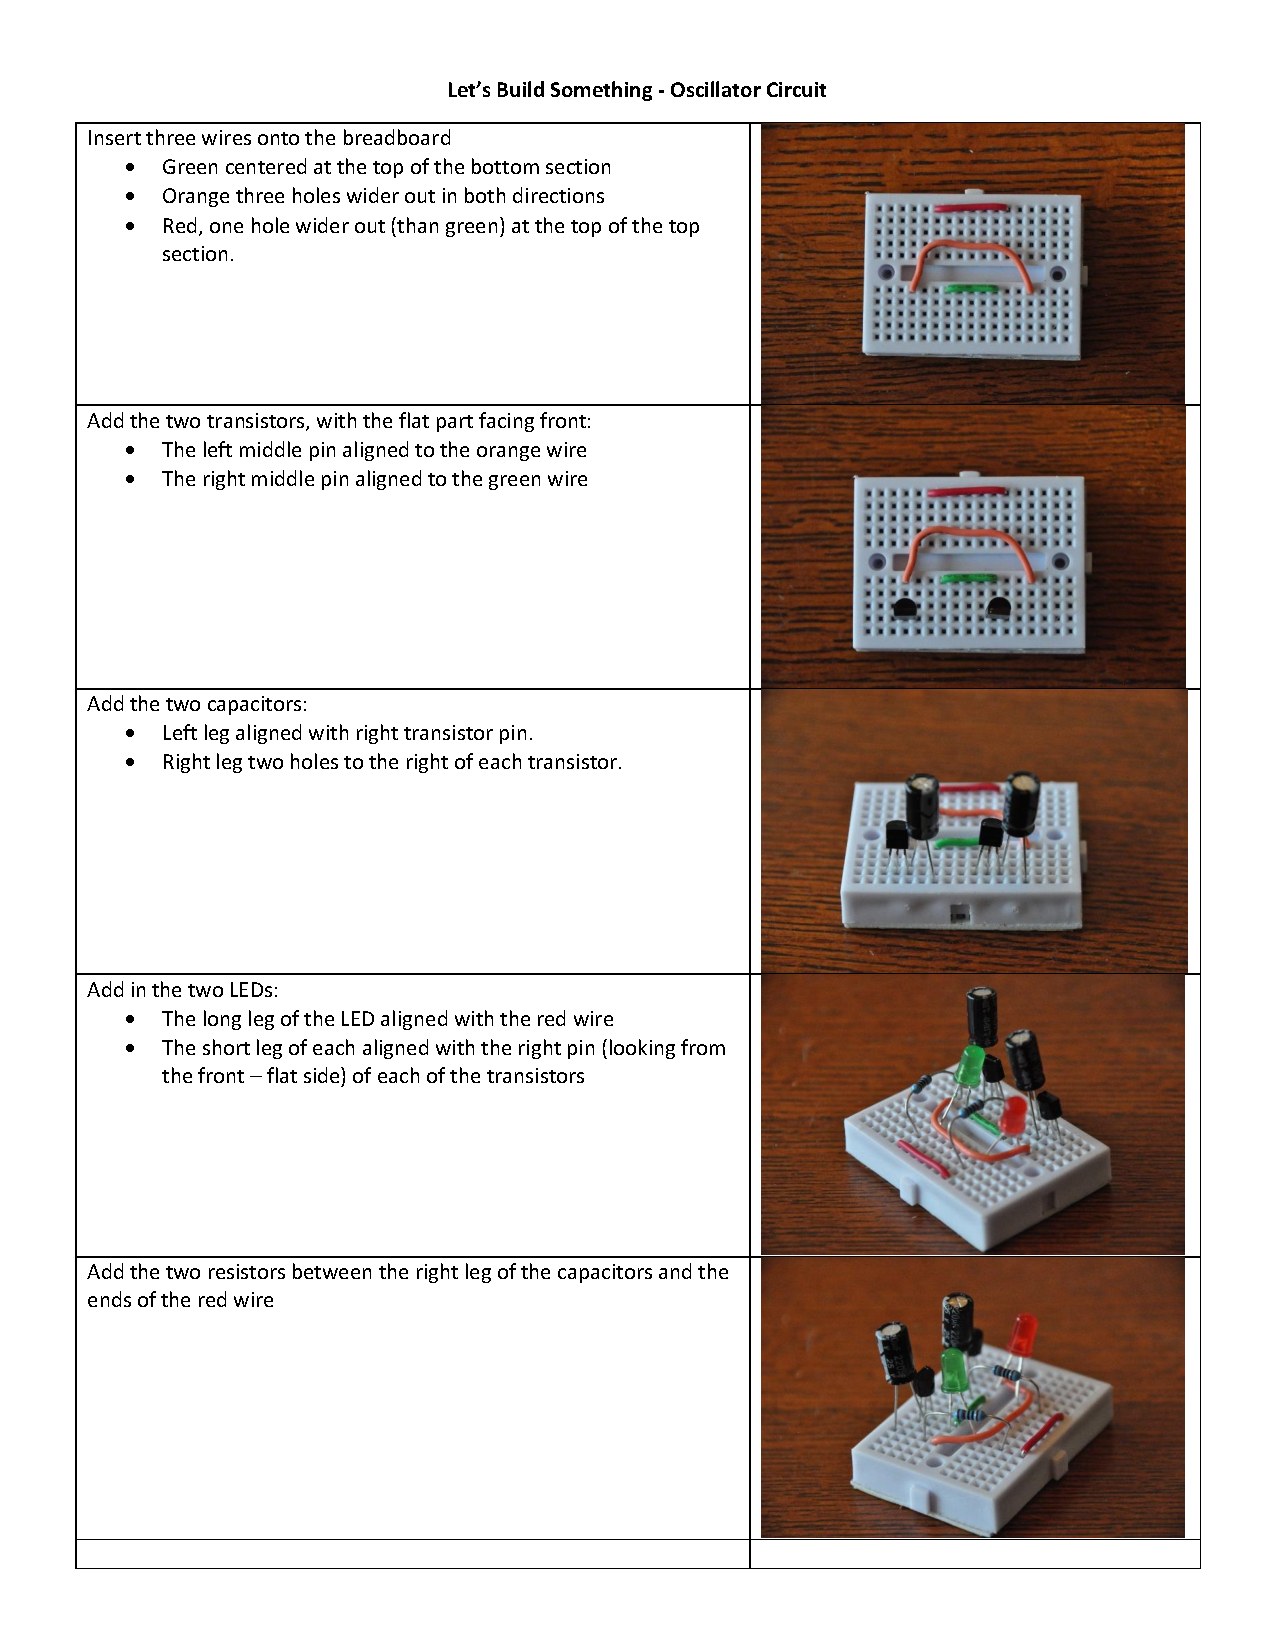
\includegraphics[scale=1.2]{oscillator.jpg} 
	\end{center}
\end{frame}

\begin{frame}\frametitle{Oscillator: Flip Flop}
\begin{columns}
\begin{column}{5.5cm}
	\begin{center}	
	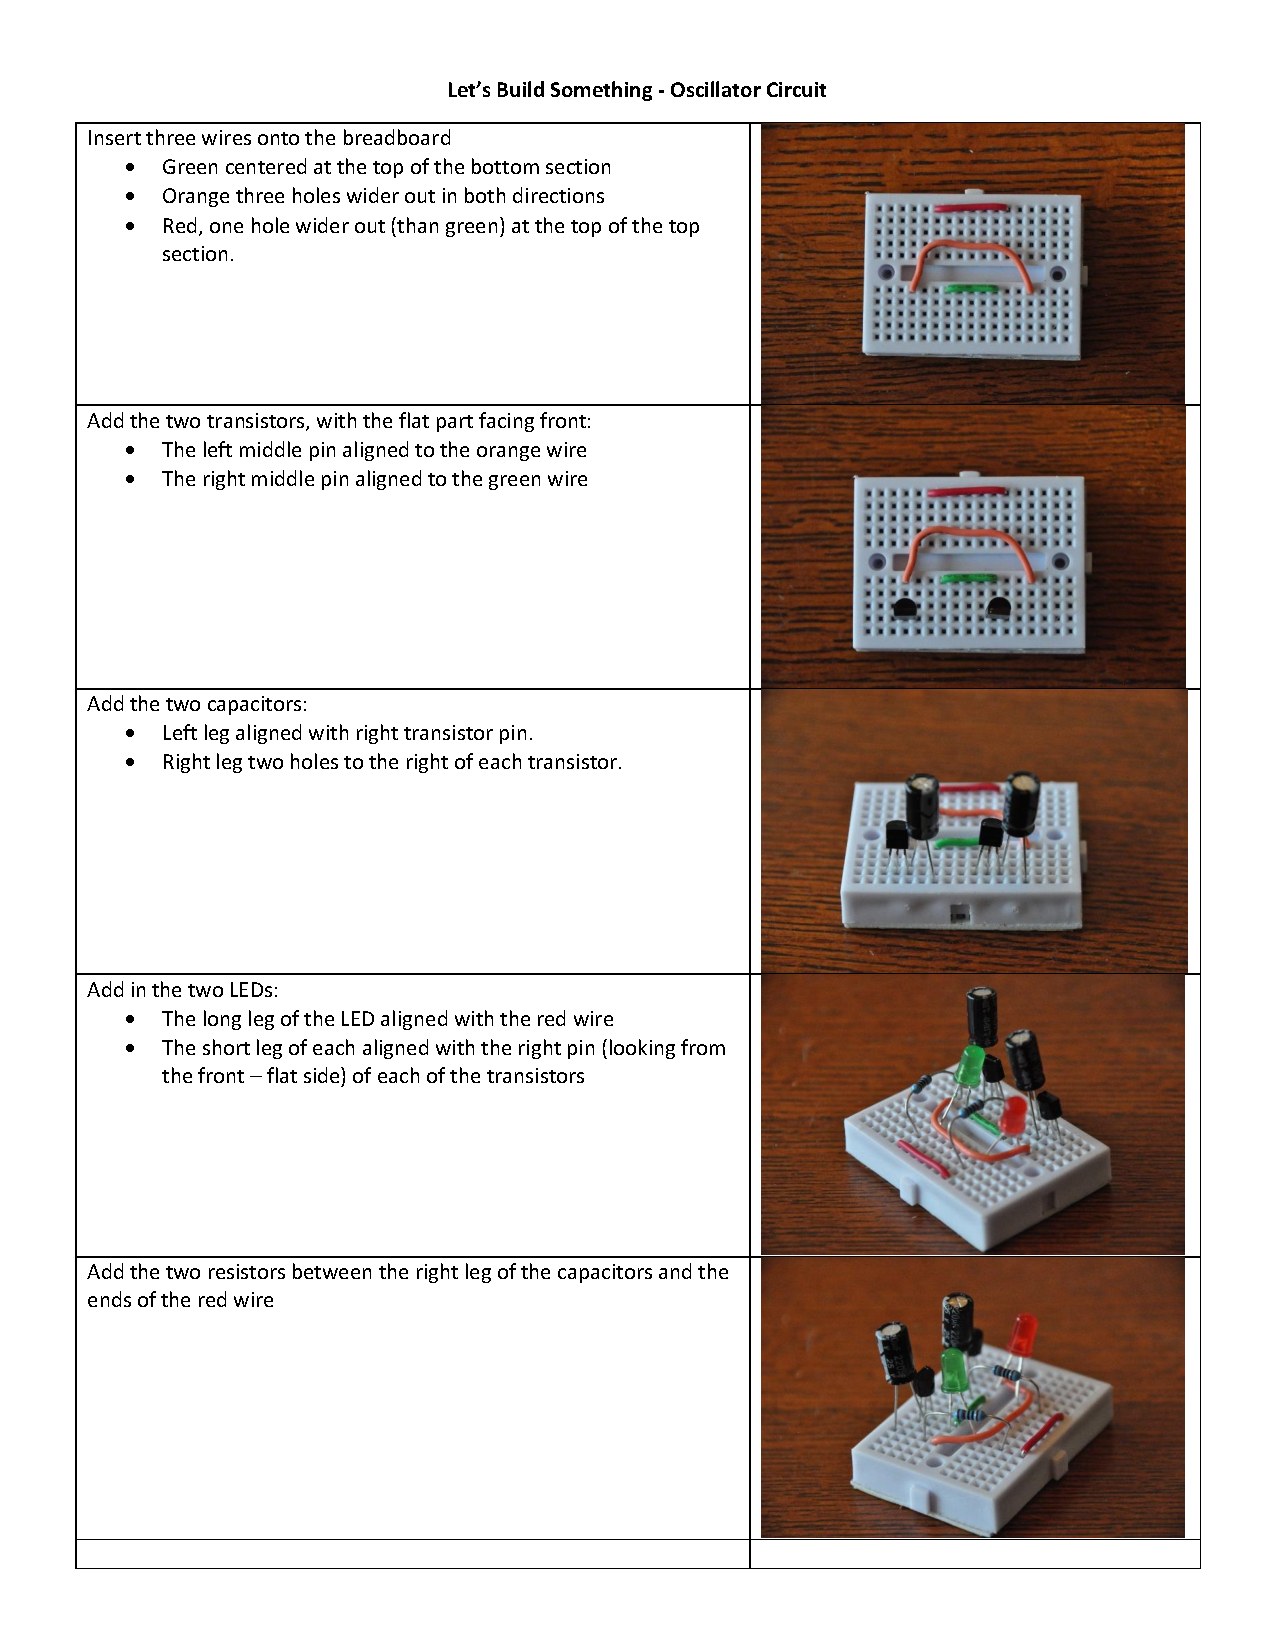
\includegraphics[scale=0.35]{oscillator.png} 
	\end{center}
\end{column}
\begin{column}{5.5cm}
Components:
\begin{itemize}
\item breadboard
\item light emitting diode (LED)
\item wires
\item resistors
\item capacitors
\item transistors
\item battery charge circuit
\end{itemize}
\end{column}
\end{columns}
\end{frame}


\begin{frame}\frametitle{Evolution of Industry}
	\begin{center}	
	\includegraphics[scale=0.2]{buildings.jpg} 
	\end{center}
\end{frame}

\begin{frame}\frametitle{Components of Industry 4.0}
\begin{figure}[h]
	\begin{center}	
	\includegraphics[scale=0.5]{industry40b.png}
	\label{fig:ind40b} 
	\end{center}
\end{figure}
\end{frame}

\begin{frame}\frametitle{IoT and Data Science}
\begin{figure}[h]
	\begin{center}	
	\includegraphics[scale=0.50]{iot-bigdata.jpg}
	\end{center}
\end{figure}
\end{frame}

\begin{frame}\frametitle{IoT 2025}
\begin{figure}[h]
	\includegraphics[scale=0.25]{9iot.png}	
\end{figure}
\end{frame}

\begin{frame}\frametitle{Smart Facilities}
\begin{figure}[h]
	\includegraphics[scale=0.30]{samrtfac.png}	
\end{figure}
\end{frame}

\begin{frame}\frametitle{Healthcare 2025}
\begin{figure}[h]
	\includegraphics[scale=0.30]{smarthealth.jpg}	
\end{figure}
\end{frame}

\begin{frame}\frametitle{Smart World}
\begin{figure}[h]
	\begin{center}	
	\includegraphics[scale=0.30]{smartwoworld.png}
	\end{center}
\end{figure}
\end{frame}

\begin{frame}\frametitle{And Out of This World}
\begin{figure}[h]
	\begin{center}	
	\includegraphics[scale=0.40]{space.jpg}
	\end{center}
\end{figure}
\end{frame}

\begin{frame}\frametitle{IoT Growth}
\begin{figure}[h]
	\begin{center}	
	\includegraphics[scale=0.42]{iot-devices2.jpg}
	\end{center}
\end{figure}

How ubiquitous is the Internet of Things?
\begin{itemize}
\item There are approximately 31 billion IoT devices today.
\item 127 new IoT devices are connected to the internet every SECOND.
\item This morning, 1,828,800 IoT devices will be added to the internet.
\end{itemize}



\end{frame}

\begin{frame}\frametitle{Let's Begin Our Journey}
\begin{figure}[h]
	\begin{center}	
	\includegraphics[scale=0.40]{divein.jpg}
	\end{center}
\end{figure}
\end{frame}


\begin{frame}\frametitle{Computer Languages}
\begin{figure}[h]
	\begin{center}	
	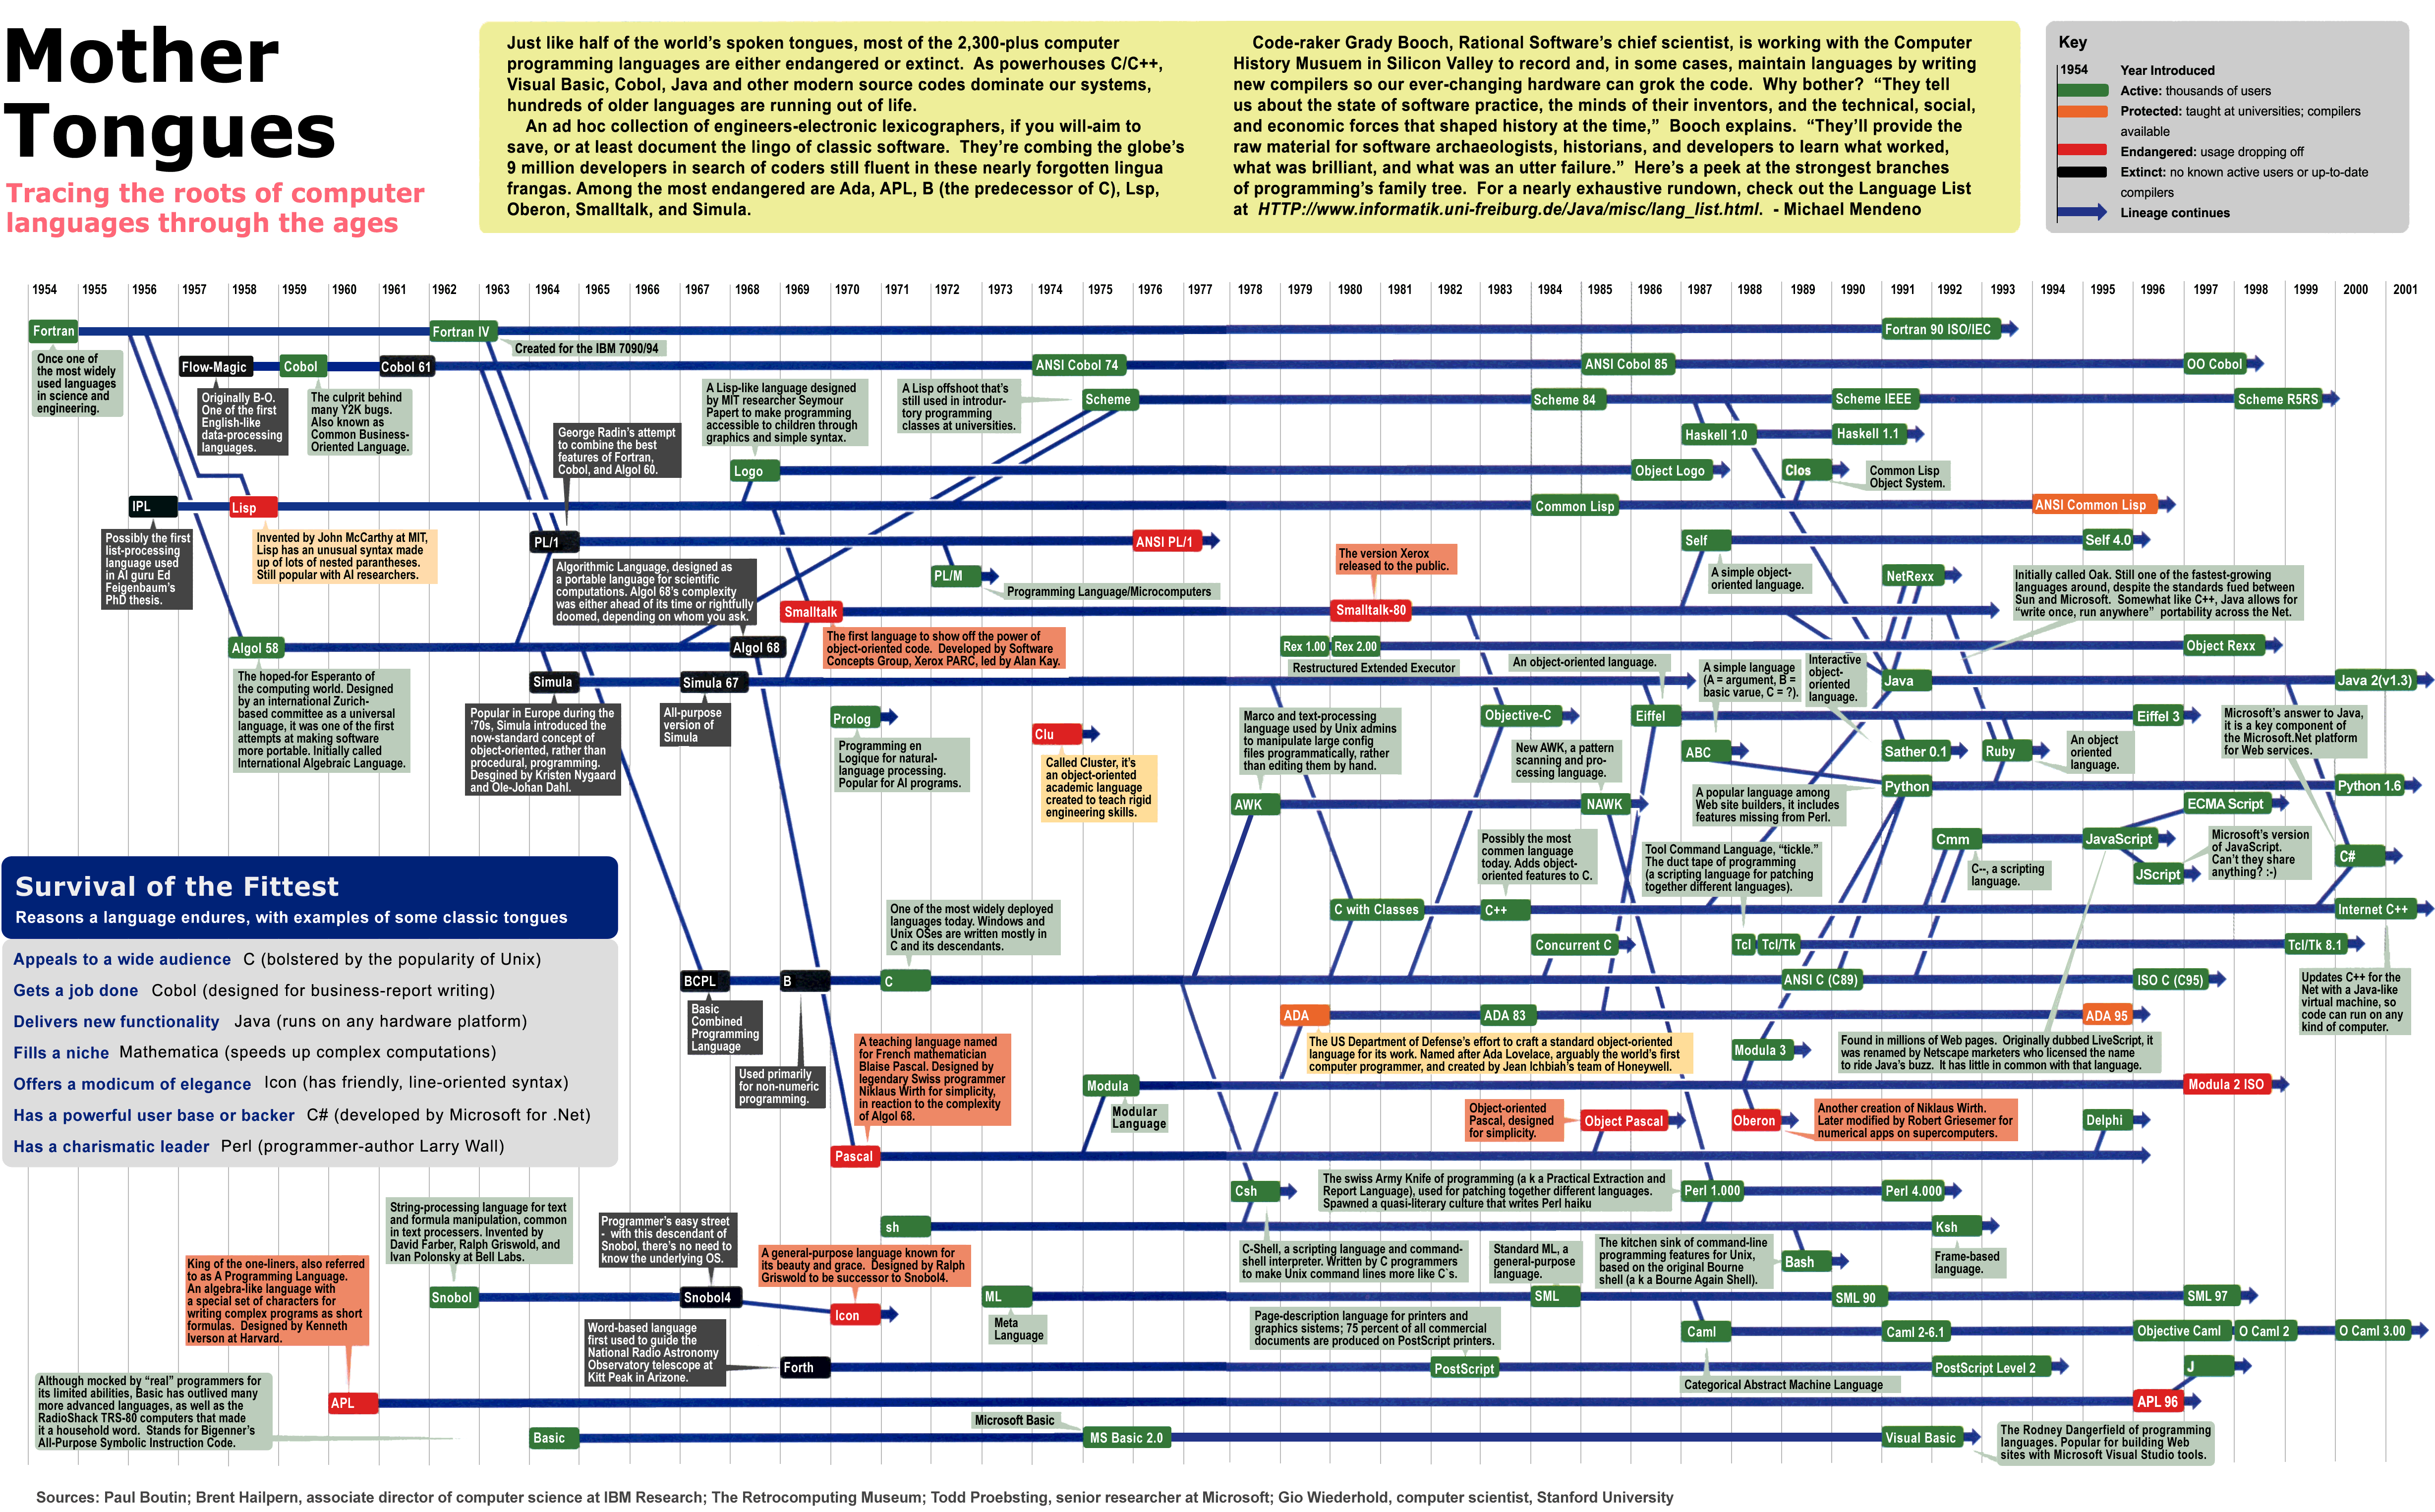
\includegraphics[scale=0.07]{ComputerLanguagesChart.png}
	\end{center}
\end{figure}
\end{frame}

\begin{frame}\frametitle{Computer Languages}
\begin{figure}[h]
	\begin{center}	
	\includegraphics[scale=0.70]{lang1.png}
	\end{center}
\end{figure}
\end{frame}

\begin{frame}\frametitle{Why C++}
\begin{figure}[h]
	\begin{center}	
	\includegraphics[scale=0.40]{whycpp.png}
	\end{center}
\end{figure}
\end{frame}

\begin{frame}\frametitle{Operating Systems}
\begin{figure}[h]
	\begin{center}	
	\includegraphics[scale=0.25]{OS_family_tree.png}
	\end{center}
\end{figure}
\end{frame}


\begin{frame}\frametitle{CLI vs GUI}
\begin{figure}[h]
	\includegraphics[scale=0.40]{guicli.png}
\end{figure}
\end{frame}


\begin{frame}\frametitle{Command Line Interface - Basic Navigation}
\label{commandlineinterface}

The Command Line Interface (CLI) will allow us to directly navigate the computers operating system. We will use:
\begin{itemize}
\item macOS or Linux: Terminal
\item Windows: PowerShell
\end{itemize}

The following commands will work on all three systems, except where noted below. macOS and Linux are case-sensitive, Windows is not.

\begin{itemize}
\item pwd: Show the present working directory.
\item ls: To get the list of all the files or folders.
\item cd: Used to change the directory.
\item du: Show disk usage. (not available in PowerShell).
\item man: Used to show the manual of any command.
\end{itemize}
\end{frame}

\begin{frame}\frametitle{Command Line Interface - File and Directory Manipulation}

\begin{itemize}
\item mkdir: Used to create a directory if it does not already exist. It accepts directory name as input parameter.
\item rmdir: Used to delete a directory if it is empty.
\item cp: This command will copy the files and directories from source path to destination path. It can copy a file/directory with a new name to the destination path. It accepts source file/directory and destination file/directory.
\item mv: Used to move files or directories. This command is similar to the cp command but it deletes a copy of the file or directory from the source path.
\item rm: Used to remove files or directories.
\item touch: Used to create or update a file. (PowerShell New-Item).
\end{itemize}
\end{frame}

\begin{frame}\frametitle{Command Line Interface - Displaying the file contents}
\begin{itemize}
\item cat: It is generally used to concatenate files. It gives the output on the standard output.
\item more: It is a filter for paging through text one screenful at a time.
\end{itemize}
The below commands are not available in PowerShell:
\begin{itemize}
\item less: Used for viewing files instead of opening the file. Similar to the "more" command but it allows backward as well as forward movement.
\item head: Used to print the first N lines of a file. It accepts N as input and the default value of N is 10.
\item tail: Used to print the last N-1 lines of a file. It accepts N as input and the default value of N is 10.
\end{itemize}

\vspace{0.25cm}
On all systems, commands can be "piped" together: ls \textbar  \: more $<file>$
\end{frame}


\begin{frame}\frametitle{IoT Fun}
\begin{figure}[h]
	\includegraphics[scale=0.40]{cartoon10.png}
\end{figure}
\end{frame}



\section{Smart Room Controller}

\begin{frame}\frametitle{Our First Microcontroller}
\begin{figure}[h]
	\includegraphics[scale=1.20]{ourmicrocontroller.jpg}
\end{figure}
\end{frame}

\begin{frame}\frametitle{Smart Room Controller}
\begin{figure}[h]
	\includegraphics[scale=0.45,angle=90]{RoomController2_bb.jpg}
\end{figure}
\end{frame}

\begin{frame}
\frametitle{Teensy 3.2}
\begin{columns}
\begin{column}{5cm}
\begin{itemize}
\item Cortex-M4 72MHz (overclocked to 96 MHz)
\item 34 GPIO pins
\item 3.3V and 5.0V operating voltages
\item 500mA of available power with USB
\end{itemize}
\vspace{1cm} 
\end{column}
\begin{column}{5cm}
\begin{overprint}
\includegraphics[scale=0.25]{teensy32.png}
\end{overprint}
\end{column}
\end{columns}
\end{frame}

\begin{frame}
\frametitle{Teensy 3.2 Schematic}
\begin{columns}
\begin{column}{4.5cm}
\begin{itemize}
\item u1: Cortex-M4
\item u2: Bootloader
\item u3: Linear Regulator
\end{itemize}
\vspace{1cm} 
\end{column}
\begin{column}{7cm}
\begin{overprint}
\includegraphics[scale=0.32]{schematic32.png}
\end{overprint}
\end{column}
\end{columns}
\end{frame}

\begin{frame}\frametitle{Arduino IDE for Teensy}
We are going to start off using the Arduino IDE\footnote{An IDE, or Integrated Development Environment, enables programmers to consolidate the different aspects of writing a computer program.}. The Arduino IDE is programmed essentailly using C++ code, but makes the compiling and loading onto the microcontroller simpler. 
\newline \newline
We begin by installing the Arduino IDE (Skip this step if on Mac): \url{https://www.arduino.cc/en/main/software}
\newline \newline
Then, we install the Teensyduino add-on: \url{https://www.pjrc.com/teensy/td\_download.html}
\newline \newline
Finally, if OneDrive is enabled, create a folder in the local Documents called Ardunio and use File $\rightarrow$ Preferences $\rightarrow$ Sketchbook location to point to this new folder.
\end{frame}

\begin{frame}\frametitle{Other Software}
\begin{enumerate}
\item Git
	\begin{itemize}
	\item For Windows - \url{https://git-scm.com/download/win}
	\item For Mac - \url{https://git-scm.com/download/mac}
	\item For Linux - sudo apt-get install git-all
	\end{itemize}
\item Fritzing
	\begin{itemize}
	\item IoT Bootcamp Teams Site
	\item Note: to extract faster, \url{https://www.7-zip.org/download.html}
	\end{itemize}
\item Drawio
	\begin{itemize}
	\item \url{https://app.diagrams.net/}
	\end{itemize}
\item Adobe Illustrator 
	\begin{itemize}
	\item \url{https://www.adobe.com/creativecloud.html} 
	\end{itemize}
\item Formlab's Preform
	\begin{itemize}
	\item \url{https://formlabs.com/software/}
	\end{itemize}
\item Ultimaker's Cura
	\begin{itemize}
	\item \url{https://ultimaker.com/software/ultimaker-cura}
	\end{itemize}
\item Bookmark: \url{https://www.desmos.com/}
\end{enumerate}
\end{frame}

\begin{frame}\frametitle{Solidworks}


To install Solidworks (Windows only), go to \url{http://www.SolidWorks.com/SEK}
\begin{itemize}
\item Enter your contact information.
\item Check the radio button “Yes” under "I already have a Serial Number that starts with 9020".
\item Select the version and click Request Download.
\item On the next page, Accept the agreement and continue.
\item On the final page, click the Download button to download the SolidWorks Installation Manager.
\item Unzip the files to launch the Installation.
\item Select the option for Individual/On this machine.
\item Install using the following serial number provided by your instructor.
\end{itemize}
macOS and Linux users will use onShape: \url{https://www.onshape.com/en/education/}
\end{frame}

\begin{comment}
Serial Number: 902000494894488736DT9M8D
\end{comment}

\section{GitHub - Part 1}
\label{githubsection1}
\begin{frame}\frametitle{Git and GitHub: Your Version Control Friends}
\begin{center}
\includegraphics[scale=0.45]{git1.png}
\end{center}
\end{frame}

\begin{frame}\frametitle{What is a version control system?}
Version Control Systems (VCS) record changes made to files so that you can
\vspace{1cm}
\begin{itemize}
\item compare and track changes over time
\item revert single files to a previous state
\item revert an entire project to an earlier version
\end{itemize}
\vspace{1cm}
Git is a VCS, or Version Control System.\newline
It is similar to Backup on Windows or Time Machine on the Mac.
\end{frame}

\begin{frame}\frametitle{Installing Git}
If you have not already done so, install Git on your computer.
\vspace{1cm}
\begin{itemize}
\item For Windows - \url{https://git-scm.com/download/win}
\item For Mac - \url{https://git-scm.com/download/mac}
\item For Linux - sudo apt-get install git-all
\end{itemize}
\vspace{1cm}
\emph{Note: For Mac, if you have XCode installed, then you will already have Git. To verify, you can type git --version in terminal.}
\end{frame}

\begin{frame}\frametitle{Why use a version control system?}
Before Version Control Systems.
\begin{itemize}
\item Save multiple versions of the file and try to remember which is which.
\item Run a text comparison tool to see what changed between versions.
\item Work with system engineer to get your changes merged with production version.
\end{itemize}
With Git.
\begin{itemize}
\item Commit as you code.
\item Versioning and timestamping automatically happen.
\item Easy to see differences between versions using git diff or visually if using GitHub.
\item Easy to merge changes to production or rollback versions.
\item Links with ticketing system for better task management and customer support.
\end{itemize}
\end{frame}

\begin{frame}\frametitle{Git vs. GitHub}
Git is the version control system. This is on your \textbf{local system}.\newline\newline
GitHub is a GUI (Graphical User Interface) \textbf{cloud-based} product that allows you to save your work remotely and facilitates collaboration.\newline\newline
\end{frame}

\begin{frame}\frametitle{Commit vs. Push}
To save files to your  \textbf{LOCAL} repository. use the \emph{commit} command. The file is given a timestamp and a unique commit number that is the file version.\newline\newline
$\rightarrow$ git commit\newline\newline
To save a file to your \textbf{REMOTE} GitHub repository, use the \emph{push} command.\newline\newline
$\rightarrow$ git push\newline\newline
\color{red}
Remember to Push your files
\color{black}
in order to save from data loss and to ensure your work is available for collaboration.
\end{frame}

\begin{frame}\frametitle{When should you commit and push your work?}
When to commit? \color{red}\textbf{OFTEN!}\color{black}
\begin{itemize}
\item Any time you finish a task where you want to save or retain a version.
\end{itemize}
\vspace{1cm}
When to push? \color{red}\textbf{OFTEN!}\color{black}
\begin{itemize}
\item Any time you have finished a task, milestone, or significant project.
\item At the end of each work session
\begin{itemize}
\item Before you take a break
\item Before a meeting
\item Before lunch
\item Before you go offline for the day
\end{itemize}
\end{itemize}
\end{frame}

\begin{frame}\frametitle{Getting a GitHub account}
If you do not already have a GitHub account, you will want to create one. 
\vspace{1cm}
\begin{enumerate}
\item Go to \url{https://github.com}
\item Click Sign Up.
\item Type a unique username and password for your account. 
\begin{itemize}
\item \emph{Note: you should consider a user name that is professional if you plan to share your GitHub account with prospective employers as part of your work portfolio.}
\end{itemize}
\item Complete the sign up process and Create Account.
\end{enumerate}
\end{frame}

\begin{frame}\frametitle{GitHub Authentication: Using HTTPS and PAT}
Effective August 2021, account passwords will no longer be allowed for command line GitHub access. Instead, you must create a Personal Access Token (PAT) to use in place of a less secure password.\newline\newline
To create a PAT:
\begin{enumerate}
\item Login to your GitHub account.
\item Click your account icon.
\item Click the Settings menu option.
\item Click Developer Settings.
\item Click Personal access tokens.
\item Generate a new token for GitHub Command Line Access.
\item Check the repo option.
\item Click Generate Token.
\end{enumerate}
\vspace{0.25cm}
Now when you login to GitHub on the command line, use your PAT rather than your password to access your account.\newline\newline
\url{https://docs.github.com/en/github/authenticating-to-github/creating-a-personal-access-token}
\end{frame}

\begin{frame}\frametitle{GitHub Authentication: Switching from password to PAT}
If you have been connecting to GitHub from the command line using your password, you will need to switch to using your Personal Access Token (PAT). \newline\newline
On Windows 10:
\begin{enumerate}
\item Open Credential Manager.
\item Click Windows Credentials.
\item Delete the git:https://github.com entry.
\end{enumerate}
\vspace{0.25cm}
On Mac OSx:
\begin{enumerate}
\item Open Keychain Access application.
\item Search for github.
\item Delete github entries as desired.
\end{enumerate}
\vspace{0.25cm}
The next time you attempt a git command on the command line,  you will be prompted to enter your username and password or PAT. If you have trouble authenticating with PAT, check that your version is at least 2.30.
\end{frame}

\begin{frame}\frametitle{Using Git: Command line or GUI?}
Why should I use the command line when I could use a GUI instead?
\begin{itemize}
\item It's generally better supported than GUI-based tools.
\item It's independent from your IDE.
\item It helps you come to a better understanding of the principles of version control.
\item It's much more commonly used in the industry and thus is more likely to get you a job.
\item It's much more likely to be useful if you find yourself in a sticky merge/rebase situation that you can't seem to fix.
\item It’s faster to type the commands than to go through the GUI. These time savings add up.
\end{itemize}
\end{frame}

\begin{frame}\frametitle{The command line}
Windows
\begin{itemize}
\item PowerShell - \color{red}This is what we are using in class.\color{black}
\item GitBash - Linux commands and editors available.
\end{itemize}
\vspace{1cm}
Mac or Linux
\begin{itemize}
\item Terminal - \color{red}This is what our Mac users are using in class.\color{black}
\end{itemize}
\vspace{1cm}
For basic commands, review IoT slides on \hyperlink{commandlineinterface}{\emph{Command Line Interface}}.
\end{frame}

\defverbatim[colored]\lstNa{
\begin{lstlisting}[language=bash,basicstyle=\ttfamily\tiny,keywordstyle=\color{red}]
brian:~$ cd Documents/
brian:Documents$ mkdir IoT
brian:Documents$ cd IoT
brian:IoT$ git clone https://github.com/ddc-iot/L01_helloWorld-brashap
Cloning into 'L01_helloWorld'...
Username for 'https://github.com': brashap
Password for 'https://brashap@github.com': 
	remote: Enumerating objects: 4, done.
	remote: Counting objects: 100% (4/4), done.
	remote: Compressing objects: 100% (3/3), done.
	remote: Total 4 (delta 0), reused 4 (delta 0), pack-reused 0
	Unpacking objects: 100% (4/4), 321 bytes | 53.00 KiB/s, done.
\end{lstlisting}
}

\begin{frame}{GitHub: Cloning and Pulling Code}
To get an existing GitHub repository, you will clone it to your local system.\newline\newline
\textbf{git clone \textless URL of repository\textgreater }\newline\newline
To get updates from a GitHub repository after you have already cloned it to your local system, you will pull the code.\newline\newline
\textbf{git pull}\newline\newline
\emph{Note: make sure you are in the repository folder before doing a git pull.}
\end{frame}

\begin{frame}{GitHub: Getting Class Slides}
You will need a copy of the class slides repository. To get class slides:\newline\newline
git clone \url{https://github.com/ddc-iot/class\_slides}\newline\newline
\emph{Note: Every morning remember to pull a copy of the class slides so that you have the latest copy.}
\end{frame}

\begin{frame}{GitHub: Getting Assignments}
\begin{columns}
\begin{column}{5cm}
\begin{overprint}
\includegraphics[scale=0.25]{gt01.png}
\end{overprint}
\end{column}
\begin{column}{5cm}
\begin{overprint}
\includegraphics[scale=0.25]{gt02.png}
\end{overprint}
\end{column}
\end{columns}

\lstNa
\end{frame}

\defverbatim[colored]\lstN{
\begin{lstlisting}[language=C++,basicstyle=\ttfamily,keywordstyle=\color{red}]
// In PowerShell go to ./Documents/IoT
// Get a repository that already exists and pull it into your local machine
	git clone <URL of repository>

// Send your changes up to the repository
	git add .	//adds all changed files
	git commit -m "some comment"
	git push	//send your changes to the cloud
	
// The first time you use git, you may get asked to enter your GIT username
git config --global user.email "you@example.com"

// From the repository directory, get updates
	git pull
\end{lstlisting}
}

\begin{frame}{GitHub: Cheatsheet. Memorize this!}
\lstN
\end{frame}

\section{L01\_HelloWorld}

\begin{frame}
\frametitle{Teensy on Breadboard}
\begin{columns}
\begin{column}{4cm}
\begin{center}
\includegraphics[scale=0.40]{teensy32_bb.png} 
\end{center}
\end{column}
\begin{column}{7.5cm}
\begin{center}
Horizontal Rows

\vspace{0.25cm}

\includegraphics[scale=0.25]{bb1.png} 
\includegraphics[scale=0.25]{bb2.png}

\vspace{0.5 cm}

Vertical Columns

\vspace{0.25cm}

\includegraphics[scale=0.25]{bb3.png} 
\includegraphics[scale=0.25]{bb4.png}
\end{center}
\end{column}
\end{columns}
\end{frame}

\defverbatim[colored]\lsta{
\begin{lstlisting}[language=C++,basicstyle=\ttfamily,keywordstyle=\color{red}]
// the "header" is used for GLOBALS

void setup() {
	// code in setup() runs once
	// it is used to initialize objects, 
	// begin processes, and set variables  
	pinMode(13, OUTPUT);	//set Pin 13 as an Output
}

void loop() {
  // functionality of your code
  // this loops indefinitely
}
\end{lstlisting}
}

\begin{frame}{Basic Structure of Arduino Sketch}
\lsta
\end{frame}

\defverbatim[colored]\lstb{
\begin{lstlisting}[language=C++,basicstyle=\ttfamily,keywordstyle=\color{red}]
/*
 * Project:     Title of Project
 * Description: Description of Project
 * Author:      Your Name
 * Date:        Today's Date
 */
 
// Single Line Comments
\end{lstlisting}
}

\begin{frame}{Class Assignments}
\begin{enumerate}
\item Lab Notebook - flow chart
\item Lab Notebook - schematic
\item Fritzing breadboad layout
\item Arduino code with comments
\lstb
\end{enumerate}
\end{frame}

\begin{frame}\frametitle{Hello World in some of the 603+ Coding Languages}
\begin{figure}[h]
	\includegraphics[scale=0.34]{sayhello.jpg}
\end{figure}
\end{frame}

\begin{frame}
\frametitle{Assignment L01\_01\_HelloWorld}
\begin{columns}
\begin{column}{4cm}
\begin{overprint}
\includegraphics[scale=0.15]{assignment.png}
\end{overprint}
\end{column}
\begin{column}{6cm}
We will write our first program together as a class, using:
\begin{itemize}
\item pinMode(pin,mode)
\item digitalWrite(pin,state)
\item delay(delay\_time)
\end{itemize}
\end{column}
\end{columns}

\vspace{0.5cm}

How fast can you make it blink and still see it blinking?
\end{frame}

\section{L02\_HelloLED}

\defverbatim[colored]\lstasc{
\begin{lstlisting}[language=C++,basicstyle=\ttfamily\tiny,keywordstyle=\color{red}]
void setup() {
	Serial.begin(9600);
	Serial.printf("Hello World! \n");
}

void loop() {}
\end{lstlisting}
}

\defverbatim[colored]\lstass{
\begin{lstlisting}[language=bash,basicstyle=\ttfamily\tiny,keywordstyle=\color{red}]
HelloWorld.bin:     file format binary
Disassembly of section .data:
00000000 <.data>:
    101c:	bd10      	pop	{r4, pc}
    101e:	4402      	add	r2, r0
    1020:	4603      	mov	r3, r0
    1022:	4293      	cmp	r3, r2
    1024:	d002      	beq.n	0x102c
    1026:	f803 1b01 	strb.w	r1, [r3], #1
    102a:	e7fa      	b.n	0x1022
    102c:	4770      	bx	lr
    102e:	0000      	movs	r0, r0
    1030:	b538      	push	{r3, r4, r5, lr}
\end{lstlisting}
}

\begin{frame}
\frametitle{Rubber Ducking - An Odd but Brilliant Tool}
\begin{figure}
\includegraphics[scale=0.20]{duck.jpg} 
\end{figure}

Rubber ducking is simply a method of debugging code. Programmers carry around a rubber duck with them, When they get stuck, they explain their code line-by-line to the rubber duck. 
\end{frame}

\begin{frame}
\frametitle{Introduction to Electrical Circuits}
\begin{figure}
\includegraphics[scale=0.15]{circuits2.jpg} 
\end{figure}
\end{frame}


\begin{frame}
\frametitle{Energy}
\begin{figure}
\includegraphics[scale=0.15]{EnergyAlien.jpg} 
\end{figure}
\begin{itemize} 
\item Kinetic Energy - energy of motion
\item Potential Energy - energy stored in an object
\end{itemize}
\end{frame}

\begin{frame}\frametitle{Electrical Circuit Terms}
\begin{figure}
\includegraphics[scale=0.50]{terms.png} 
\end{figure}
\end{frame}


\begin{frame}\frametitle{Ohm's Law}
Georg  Ohm (16 March 1789 – 6 July 1854) was a German physicist and mathematician. As a school teacher, Ohm began his research with the new electrochemical cell, invented by Italian scientist Alessandro Volta. Ohm found that there is a direct proportionality between the potential difference (voltage) applied across a conductor and the resultant electric current. This relationship is known as Ohm's law:
\vspace{0.5cm}
\begin{columns}
\begin{column}{5.5cm}
\includegraphics[scale=0.33]{ol2.jpg}
\end{column}
\begin{column}{5.5cm}
\includegraphics[scale=.1]{Volt_Amp_Ohm.png}
\end{column}
\end{columns}
\end{frame}

\begin{frame}
\frametitle{Resistor Color Bands}
\begin{figure}
\includegraphics[scale=0.40]{resistor_colors.png} 
\end{figure}
\end{frame}

\begin{frame}
\frametitle{Measuring Voltage, Current, and Resistance}
\begin{figure}
\includegraphics[scale=0.65]{multi1.jpg} 
\includegraphics[scale=0.38]{multi2.jpg} 
\end{figure}
\end{frame}

\begin{frame}
\frametitle{Power from the Teensy 3.2}
\begin{figure}
\includegraphics[scale=0.6]{02_breadboard_bb.jpg} 
\end{figure}
The Teensy 3.2 has three pins related to power:
\begin{itemize}
\item 3.3V: 250mA of power to be used for most hardware
\item $V_{in}$:  5V from the USB cable to power 5V hardware
\item GND:  The ground pin to close the electrical loop
\end{itemize}
\end{frame}

\begin{frame}
\frametitle{One Resistor}
\begin{figure}
\includegraphics[scale=0.65]{02_resistors_bb1.jpg} 
\end{figure}

\vspace{1.0cm}

Using your multimeter, measure the voltage "across" and current "through" the resistor.
\end{frame}

\begin{frame}
\frametitle{Kirchhoff's First Law}
Gustav Robert Kirchhoff (12 March 1824 – 17 October 1887) was a German physicist who contributed to the fundamental understanding of electrical circuits. His first law:
\begin{columns}
\begin{column}{5cm}
In an electrical circuit, the sum of currents flowing into that node is equal to the sum of currents flowing out of that node
\end{column}
\begin{column}{4cm}
\begin{overprint}
\includegraphics[scale=0.25]{KFL2.png}
\end{overprint}
\end{column}
\end{columns}
\end{frame}

\begin{frame}
\frametitle{Kirchhoff's Second Law}
\begin{columns}
\begin{column}{4cm}
The directed sum of the potential differences (voltages) around any closed loop is zero.
\end{column}
\begin{column}{6cm}
\begin{overprint}
\includegraphics[scale=0.25]{KSL2.png}
\end{overprint}
\end{column}
\end{columns}
\end{frame}

\begin{frame}
\frametitle{Kirchhoff's Second Law}
\begin{figure}
\includegraphics[scale=0.40]{klooplaw.jpg} 
\end{figure}
\end{frame}


\begin{frame}
\frametitle{Resistors in Series and Parallel}
\begin{figure}
\includegraphics[scale=0.40]{SP.png} 
\end{figure}
\end{frame}

\begin{frame}
\frametitle{Resistors in Series and Parallel}
\begin{columns}
\begin{column}{5cm}
\begin{center}
\includegraphics[scale=0.25]{series.png}

\vspace{0.5cm}

$R_{eq} = R_1+R_2+R_3$
\end{center}
\end{column}
\begin{column}{5cm}
\begin{center}
\includegraphics[scale=0.25]{parallel.png}

\vspace{0.5cm}

$\frac{1}{R_{eq}} = \frac{1}{R_1}+\frac{1}{R_2}$
\end{center}
\end{column}
\end{columns}
\end{frame}

\begin{frame}\frametitle{Resistors in Series}
\begin{columns}
\begin{column}{5cm}
\begin{center}
\includegraphics[scale=0.25]{series.png}

\vspace{0.5cm}

Node Law: $I = I_1 = I_2 = I_3$

\vspace{0.2cm}

Loop Law: $V_{cc} - (V_1 + V_2 + V_3) = 0$

\end{center}
\end{column}
\begin{column}{5cm}

\begin{equation}
V_{cc} = V_1 + V_2 + V_3
\end{equation}

\begin{equation}
V_{cc} = I R_1 + I R_2 + I R_3
\end{equation}

\begin{equation}
V_{cc} = I (R_1 + R_2 + R_3)
\end{equation}

\begin{equation}
\boxed{R_{eq} = R_1 + R_2 + R_3}
\end{equation}

\end{column}
\end{columns}
\end{frame}






\begin{frame}\frametitle{Resistors in Parallel}
\begin{columns}
\begin{column}{5cm}
\begin{center}
\includegraphics[scale=0.25]{parallel.png}

\vspace{0.5cm}

Node Law: $I = I_1 + I_2$

\vspace{0.2cm}


Loop Law: $V_{cc} = V_1 = V_2$

\end{center}
\end{column}
\begin{column}{5cm}

\begin{equation}
I = I_1 + I_2
\end{equation}

\begin{equation}
I = \frac{V_1}{R_1} + \frac{V_2}{R_2}
\end{equation}

\begin{equation}
I = \frac{V_{cc}}{R_1} + \frac{V_{cc}}{R_2}
\end{equation}

\begin{equation}
\frac{V_{cc}}{R_{eq}} = V_{cc} (\frac{1}{R_1} + \frac{1}{R_2})
\end{equation}

\begin{equation}
\boxed{\frac{1}{R_{eq}} = (\frac{1}{R_1} + \frac{1}{R_2})}
\end{equation}
\end{column}
\end{columns}
\end{frame}

\begin{frame}
\frametitle{Install Fritzing - download from Teams}
\begin{center}
\includegraphics[scale=0.22]{SmartPlant_bb.jpg} 
\includegraphics[scale=0.28]{SmartPlant_schem.jpg}

\vspace{1cm}

Smart House Plant Watering System

\end{center}
\end{frame}

\begin{frame}
\frametitle{Assignment: L02\_00\_Resistors}
\begin{figure}
\includegraphics[scale=0.25]{res3.jpg} 
\end{figure}
\begin{itemize}
\item In your lab notebook, draw the circuit diagrams
	\begin{enumerate}
	\item Series:   $5.1k\Omega$ and $1.2k\Omega$
	\item Parallel: $5.1k\Omega$ and $1.2k\Omega$
	\item Combined: Two parallel $5.1k\Omega$ in series with $1.2k\Omega$
	\end{enumerate}
\item Calculate the combined resistance, the voltage at each node, and the current through each component.
\item Create Fritzing diagram.
\item Build \textbf{(one at a time)} on your breadboard and test your calculations with a multimeter.
\end{itemize}
\end{frame}


\begin{comment}

\begin{frame}
\frametitle{Schematics in Fritzing}
\begin{figure}
\includegraphics[scale=0.7]{L01_Resistors_schem.jpg} 
\end{figure}
In Fritzing, go to the Schematic tab and layout your resistors.

\emph{Note: The schematic for the Teensy does not match it's physical layout.}
\end{frame}

\end{comment}




\begin{frame}\frametitle{Diodes}
The key function of a diode is to control the direction of current-flow. Current passing through a diode can only go in one direction, called the forward direction. Current trying to flow the reverse direction is blocked. \newline 
\begin{columns}
\begin{column}{5cm}
\includegraphics[scale=0.25]{idealdiode.png}
\end{column}
\begin{column}{5cm}
\includegraphics[scale=0.25]{actualdiode.png}
\end{column}
\end{columns}
\end{frame}

\begin{frame}
\frametitle{Light Emitting Diodes}
LEDs (that's "ell-ee-dees") are a particular type of diode that convert electrical energy into light.
\begin{figure}	
	\includegraphics[scale=1.0]{LEDs.png}
\end{figure}
\end{frame}

\begin{frame}
\frametitle{Current Limiting Resistors}
As an LED has very little resistance, when it is connected directly to a power supply, the current draw will exceed its specifications and it will burn out. 
\newline

\begin{center}
$
V_{pp} - V_{LED} = IR \Longrightarrow 
R >= \frac{V_{pp} - V_{LED}}{I_{max}}
$
\end{center}

For a 3.3V power supply, a 0.43V across the LED, and a max current of 100mA, the resistor needs to be greater than 29$\Omega$.

\begin{figure}
	\begin{center}	
	\includegraphics[scale=.2]{curlimres2.png}
	\label{fig:CLR} 
	\end{center}
\end{figure}
\end{frame}



\begin{frame}
\frametitle{Assignment L02\_01\_helloLED}
\begin{figure}
\includegraphics[scale=0.50]{L02_helloLED_bb.jpg} 
\end{figure}
\begin{itemize}
\item Using Pin 5 as an output and the appropriate current limiting resistor, blink the LED once per second.
\item Measure the voltage at both leads of the LED and record the voltage in your notebook. 
\item Change the resistor to $1k\Omega$ and then $10k\Omega$. What happens to the brightness? Measure the voltage and current in each case. Record in your notebook.
\end{itemize}
\vspace{0.5cm}
\textbf{REMEMBER:} Lab notebook, Fritzing, breadboard, then code
\end{frame}

\begin{frame}\frametitle{Constants and Variables}
It is often useful to give a name to something that will be used repeatedly in the code. Such items can be constants or variables:
\begin{itemize}
\item A \textbf{Constant} is a declaration that does not change throughout the code. For example, the pin that an LED is attached to.
\item A \textbf{Variable} is a declaration that changes as the code processes. For example, a counter or index. 
\end{itemize}
The use of Constants and Variables has several advantages:
\begin{itemize}
\item It improves readability by assigning names to items.
\item Items can be changed by editing a single declaration.
\item It allows the code to do math.
\end{itemize}
The first two Data Types that we will be using:
\begin{itemize}
\item \textbf{int}: an Integer between $\pm 2,147,483,648$.
\item \textbf{float}: a Floating point number with 7-digits precision.
\end{itemize}
\end{frame}


\defverbatim[colored]\lstoper{
\begin{lstlisting}[language=C++,basicstyle=\ttfamily\tiny,keywordstyle=\color{red}]
// Assignment
x = y;      // assign x to be equal to y

// Math Operators
sum = x + y;
difference = x - y;
product = x * y;
quotient = x / y;
remainder = x % y;

// Incrementing
i = i + 1;
i += 1;
i++;

// Decrementing
i = i - 1;
i -= 1;
i--; 

// Comparison
(x == y);	// true if x is equal to y
(x != y);   // true if x is not equal to y
(x > y);    // true if x is greater than y
(x >= y);   // true if x is greater than or equal to y
(x < y);    // true if x is less than y
(x <= y);   // true if x is less than or equal to y

\end{lstlisting}
}



\begin{frame}\frametitle{Operators}
There are a number of operators that act on variables:
\lstoper
\end{frame}


\defverbatim[colored]\lstcv{
\begin{lstlisting}[language=C++,basicstyle=\ttfamily,keywordstyle=\color{red}]
const int LEDPIN = 5;
const int LEDDELAY = 1000;
int i;

void setup() {          
	pinMode(LEDPIN, OUTPUT);//set LEDPIN as Output
	i = 100;
}
void loop() {              
	digitalWrite(LEDPIN,HIGH);
	delay(LEDDELAY);
	digitalWrite(LEDPIN,LOW);
	delay(LEDDELAY+i);
	i = i + 100;
}
\end{lstlisting}
}

\begin{frame}\frametitle{Constants and Variables Example}
\lstcv
\end{frame}



\begin{frame}\frametitle{Assignment L02\_02\_helloLEDvar}
\begin{columns}
\begin{column}{4cm}
\begin{center}
\includegraphics[scale=0.30]{ref.png}
\end{center}
\end{column}
\begin{column}{6cm}
\begin{itemize}
\item Refactor your L02\_01\_helloLED code to use constants and/or variables.
\end{itemize}
\end{column}
\end{columns}

\vspace{.5cm}

\emph{Note: refactoring code is when you rewrite portions of your code to make it more readable, or to make it run more efficiently.}
\end{frame}

\begin{frame}\frametitle{IoT Style Guide - camelCase}
\begin{center}
\includegraphics[scale=0.12]{camel.png}
\end{center}

Camel Case is the practice of writing phrases without spaces or punctuation, indicating the separation of words with a single capitalized letter, and the first word starting with either case. In IoT, we will start the first word as lowercase and subsequent words with upper case to delineate words. 
\end{frame}


\begin{frame}\frametitle{Pulse Width Modulation}
\begin{columns}
\begin{column}{5.5cm}
Software Configurable:
\begin{itemize}
\item Digital Input: High/Low (3.3V/0V)
\item Digital Output: High/Low (3.3V/0V)
\item Analog Input: 0V to 3.3V
\item Analog Output: 0V to 3.3V PWM
\end{itemize}
\end{column}
\begin{column}{4cm}
\begin{overprint}
\includegraphics[scale=0.20]{pwm.jpg}
\end{overprint}
\end{column}
\end{columns}
\end{frame}


\begin{frame}\frametitle{Assignment L02\_03\_helloLEDanalog}
\begin{columns}
\begin{column}{4cm}
\begin{overprint}
\includegraphics[scale=0.15]{assignment.png}
\end{overprint}
\end{column}
\begin{column}{6cm}
Use analogWrite to change the brightness of the LED, using values:
\begin{itemize}
\item 255
\item 63
\item 171
\item 16
\end{itemize}
Measure the voltage with your multimeter at each value.
\end{column}
\end{columns}

\vspace{1cm}

Syntax: analogWrite(pin,value);
\begin{itemize}
\item pin: the pin to write to
\item value: the duty cycle of the pulses, an int between 0 (always off) and 255 (always on) 
\end{itemize}
\end{frame}


\begin{frame}
\frametitle{Flowcharts}
\begin{figure}
\includegraphics[scale=0.40]{flowchart.png} 
\end{figure}
\end{frame}

\begin{frame}
\frametitle{Loops}
\begin{center}
\includegraphics[scale=0.40]{loops.jpg} 
\end{center}
\end{frame}


\defverbatim[colored]\lstII{
\begin{lstlisting}[language=C++,basicstyle=\ttfamily,keywordstyle=\color{red}]
// FOR loop syntax
for (initialization; condition; increment) {
  // statement(s);
}

// EXAMPLE
for (j=0; j <= 255; j++) {
	analogWrite(LEDPIN, j);
}
\end{lstlisting}
}
\begin{frame}{FOR Loop syntax}
\lstII
\vspace{0.50cm}
\emph{Note: the third parameter of a FOR loop can also decrement; i.e. $j--$ or can go up or down by a specified amount; i.e. j = j + 2}
\end{frame}


\defverbatim[colored]\lstII{
\begin{lstlisting}[language=C++,basicstyle=\ttfamily,keywordstyle=\color{red}]
// WHILE loop syntax
while (condition) {
  // statement(s)
}


// EXAMPLE
while (button == HIGH) {
	digitalWrite(LEDPIN, HIGH);
} //continue this loop until button is released
\end{lstlisting}
}
\begin{frame}{WHILE loop syntax}
\lstII
\end{frame}

\begin{frame}\frametitle{For vs While Loops}
\begin{figure}[h]
	\includegraphics[scale=1.25]{forwhile.jpg}
\end{figure}
\end{frame}

\begin{frame}\frametitle{Assignment L02\_04\_helloLEDtri}
\begin{columns}
\begin{column}{5cm}
\begin{overprint}
\includegraphics[scale=0.15]{waveform.png}
\end{overprint}
\end{column}
\begin{column}{4cm}
Using a FOR Loop, have the LEDs follow a Triangle Wave function from off to full brightness with a period of 10 seconds. 
\end{column}
\end{columns}

\vspace{0.5cm}
Before you write code, create a flow chart of the logic to create a triangle wave. 

\end{frame}

\begin{frame}
\frametitle{While or Do While}
\begin{figure}
\includegraphics[scale=0.27]{roadrunner.jpg} 
\end{figure}
\end{frame}



\begin{frame}\frametitle{Number Systems}
\begin{figure}[h]
	\includegraphics[scale=0.35]{bodh.jpg}
\end{figure}
\end{frame}


\begin{frame}\frametitle{Exponents}
\begin{columns}
\begin{column}{5cm}
\begin{center}
\includegraphics[scale=0.14]{exponents.jpg}
\end{center}
\end{column}
\begin{column}{5cm}
The rule for zero as an exponent:

\vspace{0.25cm}

Any nonzero real number raised to the power of zero is one, this means anything that looks like $x^0$ will always equal 1 if x is not equal to zero. 
\end{column}
\end{columns}
\end{frame}

\begin{frame}\frametitle{Bits, Nibbles, Bytes, and Words}
\begin{figure}[h]
	\includegraphics[scale=0.50]{nbw.png}
\end{figure}
\end{frame}

\begin{frame}\frametitle{Data Types: Numbers}
\includegraphics[scale=0.45]{datatypes.JPG}
\vspace{0.5cm}

There are $7.5 x 10^{18}$ grains of sand on Earth. A long long integer and the floating point numbers are larger than this. 
\end{frame}

\defverbatim[colored]\lsttype{
\begin{lstlisting}[language=C++,basicstyle=\ttfamily\tiny,keywordstyle=\color{red}]
int x = 3;
int y = 2;
float yf = 2.0;
float z;

//int divided by an int returns an int
z = x/y;                    // z = 1.0
z = x/yf;                   // z = 1.5
z = x / 2;                  // z = 1.0
z = x / 2.0;                // z = 1.5

//type casting used to change datatype
z = (float) x / (float) y;  // z = 1.5
z = x / (float) y;          // z = 1.5

z = (int) (x / yf);         // z = 1.0
y = x / yf;                 // y = 1


\end{lstlisting}
}

\begin{frame}\frametitle{Math Warning and Type Casting}
Be cognizant of the data type when performing math operations. 

\lsttype

Type Casting is a way to ensure that you are correctly moving between datatypes.
\end{frame}


\begin{frame}\frametitle{Pi ($\pi)$}

\begin{center}
\includegraphics[scale=0.8]{pi.png}
\end{center}

\end{frame}


\begin{frame}\frametitle{Unit Circle and Trigonometric Functions}
The Unit Circle is a circle with a radius of 1.
\begin{columns}
\begin{column}{6cm}
\begin{center}
\includegraphics[scale=0.75]{unitcircle.png}
\end{center}
\end{column}
\begin{column}{6cm}
\begin{center}
\includegraphics[scale=0.75]{unitcircle_cst.png}
\end{center}
\end{column}
\end{columns}
The Unit Circle can be used to map out the trigonometric values of sine, cosine, and tangent.
\end{frame}


\begin{frame}\frametitle{Unit Circle and the Value of $sin(\theta)$}
\begin{columns}
\begin{column}{6cm}
\begin{center}
\includegraphics[scale=0.25]{unitcircle_sin.png}
\end{center}
\end{column}
\begin{column}{6cm}
\begin{center}
\includegraphics[scale=0.75]{unitcircle_rad.png}
\end{center}
\end{column}
\end{columns}

\vspace{0.25cm}

\begin{itemize}
\item $sin(\theta)$ is the y-value of the point on the Unit Circle at angle $\theta$. 
\item In our trig functions, $\theta$ is measured in radians (rad), not degrees.
\item 360 degrees = $2 \pi$ radians.
\end{itemize}
\end{frame}

\begin{frame}\frametitle{Sine Waves}
\begin{center}
\includegraphics[scale=0.25]{sin.jpg}
\end{center}

\begin{center}
$y = A * sin(2*\pi*\nu*t) + B$
\end{center}

where A = amplitude, B = offset, $\nu$ = frequency = $\frac{1}{period}$, 

and t = time in seconds.
\end{frame}

\begin{frame}\frametitle{Header Files}
A header file is a file with the extension .h which contains C function declarations and macro definitions to be shared between several source files. There are two types of header files; those that the programmer writes and those that come with the compiler. 
\vspace{0.5cm}

Both the user and system header files are included using the preprocessing directive \#include. It has the following two forms:
\begin{itemize}
\item \#include $<file.h>$ for system header files.
\item \#include $"file.h"$ for user-created header files in the directory that contains the current code. 
\end{itemize}

An example of a system header file is the math.h header that defines various mathematical functions. 
\end{frame}

\defverbatim[colored]\lstd{
\begin{lstlisting}[language=C++,basicstyle=\ttfamily,keywordstyle=\color{red}]
#include <math.h>        // include header files
const int LEDPIN = 5;    // declare constants
float value,n;           // declare variables

void setup() {            // runs once
	pinMode(LEDPIN,OUTPUT); // system settings
	n = 0;                  // set variables
}

void loop() {             // loops indefinitely 
	value = sin(2*PI*n);
	n = n+0.25;       // move a quarter around 
	                  // the unit circle 
}
\end{lstlisting}
}
\begin{frame}\frametitle{Basic Structure of Arduino Sketch Revisited}
\lstd
\end{frame}


\begin{frame}\frametitle{Assignment L02\_05\_helloLEDsin}
\begin{columns}
\begin{column}{4.5cm}
\begin{overprint}
\includegraphics[scale=0.13]{waveform.png}
\end{overprint}
\end{column}
\begin{column}{5cm}
Use a sin() function to vary the brightness of your LED.
\begin{itemize}
\item Use math.h.
\item Function sin() takes a double as an input and returns a double.
\item Set the period to 5 seconds.
\end{itemize}
\end{column}
\end{columns}

\vspace{0.25cm}

Recall: for a sin wave: $y = A * sin(2*\pi*\nu*t) + B$

\vspace{0.25cm}

The function millis() returns milliseconds since the Teensy has been powered on. For the sine equation, use t = millis() / 1000.0. 

\vspace{0.5cm}

Why is adding the decimal after 1000 important?
\end{frame}

\section{L03\_Buttons}

\begin{frame}\frametitle{IoT Fun}
\begin{figure}[h]
	\includegraphics[scale=1.5]{cartoon2.jpg}
\end{figure}
\end{frame}


\defverbatim[colored]\lstIV{
\begin{lstlisting}[language=C++,basicstyle=\ttfamily,keywordstyle=\color{red}]
void setup() {

// Enable Serial Monitor
  Serial.begin (9600);
  while (!Serial);  // wait for Serial monitor
  Serial.println ("Ready to Go");
}

void loop() {
  for (i=0; i<=13; i++){
    Serial.print(i);
    delay(printDelay);
  }
}
\end{lstlisting}
}
\begin{frame}{Displaying to the Screen: The Serial Monitor}
\lstIV
\end{frame}

\begin{frame}{Print Statements}
\begin{enumerate}
\item Serial.print() prints data to the monitor through the serial port as human-readable text:
	\begin{itemize}
	\item Serial.print('N') prints: N
	\item Serial.print("Hello World") prints: Hello World
	\item Serial.print(78) prints: 78
	\item Serial.print(3.141592) prints 3.14
	\item Serial.print(3.141592,5) prints 3.14159
	\end{itemize}
\item Serial.println() displays the print() followed by a carriage return (\textbackslash r) or newline (\textbackslash n).
\item Serial.printf() displays a formatted print.
\end{enumerate}
\end{frame}

\defverbatim[colored]\lstpf{
\begin{lstlisting}[language=C++,basicstyle=\ttfamily\tiny,keywordstyle=\color{red}]
int count = 42;
float value = 3.14159;
Serial.printf("Print an integer %i and a float %0.4f\n",count,value);

//Output: Print an integer 42 and a float 3.1415
\end{lstlisting}
}

\begin{frame}{Format Specifiers Statements}
\begin{center}
	\includegraphics[align=c,scale=0.30]{printf2.png} 
	\includegraphics[align=c,scale=0.40]{printf.JPG} 
\end{center}

\lstpf
\end{frame}

\begin{frame}\frametitle{Assignment L03\_00\_SerialMonitor}
\begin{columns}
\begin{column}{4cm}
\begin{overprint}
\includegraphics[scale=0.15]{assignment.png}
\end{overprint}
\end{column}
\begin{column}{6cm}
\begin{enumerate}
\item Print Hello World to your monitor screen.
\item Next, display to the screen a count from 0 to 13, separated by commas, three times by using:
\begin{itemize}
\item Serial.print();
\item Serial.println();
\item Serial.printf();
\end{itemize}
\end{enumerate}
\end{column}
\end{columns}
\end{frame}

\begin{frame}\frametitle{One Pin - Many Functions}
\begin{center}
\includegraphics[scale=0.25]{GPIO0.png}

\vspace{0.25cm}
Software Programmable: Input or Output and Digital or Analog.
\end{center}
\end{frame}

\begin{frame}
\frametitle{Digital Input/Output}
Digital electronics rely on binary logic to store, process, and transmit data or information. Binary Logic refers to one of two states -- ON or OFF. This is commonly translated as a binary 1 or binary 0. A binary 1 is also referred to as a HIGH signal and a binary 0 is referred to as a LOW signal.
\begin{columns}
\begin{column}{3cm}
\begin{figure}
	\includegraphics[scale=0.4]{CMOS_Dio.png}
\end{figure}
\end{column}
\begin{column}{6cm}
\begin{itemize}
\item digitalWrite(pin,value);
\item inputValue = digitalRead(pin);
\end{itemize}

\vspace{0.5cm}
where, value equals HIGH or LOW.
\end{column}
\end{columns}
\end{frame}

\begin{frame}\frametitle{Switches}
\begin{figure}[h]
	\includegraphics[scale=0.40]{switchstate2.png}
\end{figure}
\end{frame}

\begin{frame}\frametitle{Poles and Throws}
\begin{figure}[h]
	\includegraphics[scale=0.25]{st2.jpg}
\end{figure}
\begin{itemize}
\item Poles indicates the number of circuits that one switch can control for one operation of the switch. 
\item Throws indicates the number of contact points.
\end{itemize}
\end{frame}


\begin{frame}\frametitle{A Button - SPST}
\begin{figure}[h]
	\includegraphics[scale=0.20]{SPST2.png}
\end{figure}
\end{frame}

\begin{frame}
\frametitle{Floating Inputs}
\begin{columns}
\begin{column}{5cm}
\begin{center}
	\includegraphics[scale=0.2]{floating.png}
\end{center}
\end{column}
\begin{column}{5cm}
\begin{figure}
	\includegraphics[scale=0.4]{CMOS_Dio.png}
\end{figure}
\end{column}
\end{columns}
\end{frame}


\begin{frame}\frametitle{Pull Down and Pull Up Resistors}
\begin{center}
	\includegraphics[scale=0.30]{pulldownpullup.png}

\vspace{0.5cm}
\begin{itemize}
\item What happens if the digital pin is left floating when the switch is open?
\item What happens if the pin is connected directly to GND (or $V_{cc}$) without a resistor?
\end{itemize}
\end{center}
\end{frame}

\begin{frame}\frametitle{Our First Button and Pull Down Resistors}
\begin{center}
	\includegraphics[scale=0.60]{L03_Button_bb.jpg}
\end{center}
\vspace{0.25cm}
Reading from a digital pin:
\begin{itemize}
\item inputValue = digitalRead(pin);


where
	\begin{itemize}
	\item pin is the digital pin that the button is connected to
	\item inputValue is an int (declared in the header)
	\end{itemize}
\end{itemize}

\end{frame}


\begin{frame}\frametitle{Model Based Troubleshooting}
\begin{center}
\includegraphics[scale=0.40]{mbts.PNG}
\end{center}
\end{frame}

\begin{frame}\frametitle{Assignment: Buttons}
\begin{columns}
\begin{column}{4.0cm}
\includegraphics[scale=0.1]{assignment.png}
\begin{itemize}
\item Notebook: draw circuit
\item Fritzing diagram
\item Wire your circuit
\item Write the code
\end{itemize}
\end{column}
\begin{column}{7.3cm}
Connect a button (and a multimeter to measure the voltage) to Pin 23. 
\begin{enumerate}
\item L03\_01\_button
	\begin{itemize}
		\item Use digitalRead() to input the button state.
		\item Print button state to the screen.
		\item Remove the resistor. How does this affect the button state and the voltage?
		\item Replace the pull-down resistor with a pull-up. How does the logic change?
		\begin{itemize}
		\item Not pressed: 3.3V
		\item Pressed: GND
		\end{itemize}
	\end{itemize}
\item L03\_02\_button\_input\_pullup
	\begin{itemize}
		\item Remove the pull-up resistor.
		\item Implement: pinMode(pin,INPUT\_PULLUP);
	\end{itemize}
\end{enumerate}
\end{column}
\end{columns}
\end{frame}



\defverbatim[colored]\lstbool{
\begin{lstlisting}[language=C++,basicstyle=\ttfamily\tiny,keywordstyle=\color{red}]
bool x;
bool buttonState1, buttonState2;
int y, z;

// ! (NOT) assignment function
x = !x; 			// toggle x (if x = 1, then set x = 0, and visa-versa)

// ! (NOT) comparison
if (!x) {			// if x is false
	// do something
}

// LOGICAL AND: if both pins are pressed
buttonState1 = digitalRead(PIN1);
buttonState2 = digitalRead(PIN2);
if ((buttonState1) && (buttonState2) {
	// do something
}

// LOGICAL OR: if either value is greater than zero
if (y > 0 || z > 0) {
	// do something
}
\end{lstlisting}
}


\begin{frame}\frametitle{IF-ELSE Statements}
\begin{center}
\includegraphics[scale=0.40]{if_else2.jpg}
\end{center}
\end{frame}

\defverbatim[colored]\lstIII{
\begin{lstlisting}[language=C++,basicstyle=\ttfamily,keywordstyle=\color{red}]
// IF statement SYNTAX
if (condition) {
  //statement(s)
}
else {
  // else statement(s)
}

// EXAMPLE
if (buttonState) {
	Serial.printf("Button is pressed \n");
}
else {
	Serial.printf("Button is not pressed \n");
}
\end{lstlisting}
}
\begin{frame}{IF-ELSE Statements}
\lstIII
\end{frame}


\begin{frame}\frametitle{Data Types: Boolean and Boolean Logic}
\begin{columns}
\begin{column}{4cm}
\includegraphics[scale=0.30]{booleanlogic.png}
Boolean datatype (bool) holds either a TRUE or FALSE
\end{column}
\begin{column}{6cm}
Boolean Logic Operations (condition statements)
\begin{enumerate}
\item NOT (!): true if operand is false and visa-versa
	\begin{itemize}
	\item $x =  !x$
	\end{itemize}
\item AND (\&\&): true if both operands are true
	\begin{itemize}
	\item $z = x \&\& y$
	\end{itemize}
\item OR ($\parallel$): true if either operand is true
	\begin{itemize}
	\item $z = x \parallel y$
	\end{itemize}
\end{enumerate}
\end{column}
\end{columns}
\end{frame}

\begin{frame}{Boolean Logic In Action}
\lstbool
\end{frame}

\begin{frame}\frametitle{Button and LED}
\begin{figure}[h]
	\includegraphics[scale=0.60]{L03_ButtonLED_bb.jpg}
\end{figure}
\end{frame}

\begin{frame}\frametitle{Assignment: Buttons and LEDs}
\begin{columns}
\begin{column}{3cm}
\begin{overprint}
\includegraphics[scale=0.12]{assignment.png}
\end{overprint}
Update your schematic and Fritzing
\end{column}
\begin{column}{7cm}
\begin{enumerate}
\item L03\_03\_buttonLED
\begin{itemize}
\item Add a Green LED to Pin 5 and use the button to turn the LED on/off.
\item Also, print button state to the screen
\end{itemize}
\item L03\_04\_twoButtonLED
\begin{itemize}
\item Add a second button (Pin 16) and Yellow LED (Pin 6).
\item Have each button control one LED.
\item Also, print button states to the screen.
\end{itemize}
\item Extra Credit: Modify twoButton
\begin{itemize}
\item The Green LED lights up if both buttons are pressed
\item The Yellow LED lights up if either button is pressed
\end{itemize}
\end{enumerate}
\end{column}
\end{columns}
\end{frame}

\begin{frame}
\frametitle{Resistors in Series and Parallel}
\begin{columns}
\begin{column}{5.5cm}
\begin{center}
Open Circuit Behavior

\vspace{0.25cm}

\includegraphics[scale=0.20]{vd1.png}

\vspace{0.5cm}

$V_{out} = V_{in} \frac{I R_2}{I (R_1 + R_2)} = \frac{R_2}{R_1 + R_2} V_{in}$
\end{center}
\end{column}
\begin{column}{5cm}
\begin{center}
Behavior Under Load

\vspace{0.25cm}

\includegraphics[scale=0.22]{vd2.png}

\vspace{0.5cm}

$V_{out} =  \frac{R_2 \parallel R_L}{R_1 + R_2\parallel R_L} V_{in}$
\end{center}
\end{column}
\end{columns}
\end{frame}

\begin{frame}\frametitle{Voltage Dividing}
\begin{figure}[h]
	\includegraphics[scale=0.60]{L03_analogVD_bb.jpg}
\end{figure}
We are just using the Teensy to provide Power and GND.
\begin{itemize}
\item Use various combinations of resistors between $1k \Omega$ and $22k \Omega$.
\item Calculate the Series resistance and the voltage between the two resistors in your Lab Notebook.
\item Measure with your multimeter and compare.
\end{itemize}
\end{frame}

\begin{frame}\frametitle{Potentiometer - Variable Resistor}
\begin{center}
\includegraphics[scale=0.60]{pot.png}
\end{center}
A potentiometer has 3 pins. Two terminals (the blue and green) are connected to a resistive element and the third terminal (the black one) is connected to an adjustable wiper.
\end{frame}


\begin{frame}\frametitle{Assignment L03\_05\_AnalogInput}
\begin{columns}
\begin{column}{4cm}
\begin{overprint}
\includegraphics[scale=0.80]{L03_analogIN_schem.jpg}
\end{overprint}
\end{column}
\begin{column}{6cm}
\begin{enumerate}
\item Look up the syntax of analogRead() in the Ardunio Reference. 
\item Utilize analogRead() to measure analog input across a potentiometer (voltage divider) using Pin 14. 
\item Determine the range of the analogRead() across the entire range of the potentiometer. 
\end{enumerate}
\end{column}
\end{columns}
\end{frame}

\begin{frame}\frametitle{Anatomy of a Function}
\begin{figure}[h]
	\includegraphics[scale=0.75]{FuncAnatomy.png}
\end{figure}
\end{frame}

\defverbatim[colored]\lstgls{
\begin{lstlisting}[language=C++,basicstyle=\ttfamily\tiny,keywordstyle=\color{red}]
int x;           // x is a global variable available in the entire program
void setup() {
	x = 1;
}
void loop() {
	x = addx();
}
int addx() {
   int y = 0;         // y is a local variable, resets every function call
   static int z = 0;  // z is a static local variable, maintains its value
   y = y + x;
   z = z + x;
   Serial.printf("x = %i, y = %i, and z = %i \n",x,y,z);
   return z;
}
\end{lstlisting}
}
\begin{frame}{Types of Variables}
\lstgls
\begin{enumerate}
\item Global Variables
\begin{itemize}
\item Accessible throughout the program and all functions. 
\end{itemize}
\item Local Variables
\begin{itemize}
\item Accessible only in the function.
\item Created when function is called. Destroyed when function is returned. 
\end{itemize}
\item Static Local Variables
\begin{itemize}
\item Accessible only in the function.
\item Maintains value across multiple calls of a function. 
\end{itemize}
\end{enumerate}
\end{frame}

\defverbatim[colored]\lste{
\begin{lstlisting}[language=C++,basicstyle=\ttfamily\tiny,keywordstyle=\color{red}]
/*
 * This is an example of how to use functions
 * The code below converts inches to feet
 */

const int INCHPIN=14;
int inches;
float feet;

void setup() { 
	Serial.begin(9600);  // Turn on Serial Monitor
	while(!Serial);      // Wait for Serial Monitor to be running         
	pinMode(INCHPIN,INPUT);
}

void loop() {           	
	inches = analogRead(INCHPIN);
	feet = inchestoFeet(inches);
	Serial.printf("%i inches equal %0.2f feet \n",inches, feet);
	delay(1000);
}

float inchestoFeet(int measurement) {
	float answer;			       // declare answer as a local variable
	
	answer = measurement / 12.0;
	return answer;
}
\end{lstlisting}
}
\begin{frame}{Basic Structure of Arduino Sketch with Functions}
\lste
\end{frame}

\begin{frame}\frametitle{Assignment L03\_05\_AnalogInput Revisited}
\begin{columns}
\begin{column}{4cm}
\begin{overprint}
\includegraphics[scale=0.80]{L03_analogIN_schem.jpg}
\end{overprint}
\end{column}
\begin{column}{6cm}
\begin{enumerate}
\item Modify your code by adding a function, intoVolts(), that converts the analog input value to voltage.
\item Print both the raw analogInput and the associated voltage to your screen. 
\end{enumerate}
\end{column}
\end{columns}
\end{frame}

\begin{frame}\frametitle{Optional Week 1 Review: L03\_00\_SOS}
\begin{columns}
\begin{column}{8cm}
\begin{figure}[h]
	\includegraphics[scale=0.28]{sos.jpg}
\end{figure}
\end{column}
\begin{column}{4cm}
\begin{figure}[h]
	\includegraphics[scale=0.1]{sos_image.jpg}
\end{figure}
\begin{tiny}
\begin{itemize}
\item Flowchart is in english, not code syntax
\item Wire one button and one LED to your Teensy
\item Declare the appropriate global variables and constants
\item First function: void sos
\item Second function: void flasher with parameters number of flashes, on time, off time between flashes
\item Variables within the functions should be local, not global
\end{itemize}
\end{tiny}
\end{column}
\end{columns}
\end{frame}

\section{L04\_oneButton}

\begin{frame}\frametitle{IoT Humor}
\begin{figure}[h]
	\includegraphics[scale=0.30]{cartoon3.jpg}
\end{figure}
\end{frame}

\begin{frame}\frametitle{Objects}
\begin{figure}[h]
	\includegraphics[scale=0.32]{object.png}
\end{figure}
\end{frame}

\begin{frame}\frametitle{Traffic Light}
\begin{figure}[h]
	\includegraphics[scale=0.40]{traffic.png}
\end{figure}
Let's use the traffic light to build our own Objects.
\end{frame}

\begin{frame}\frametitle{State Machine - Traffic Lights, British Style}

\includegraphics[scale=0.40]{traffic-light-sequence.jpg}

\end{frame}


\defverbatim[colored]\lstswitch{
\begin{lstlisting}[language=C++,basicstyle=\ttfamily,keywordstyle=\color{red}]
// SWITCH...CASE syntax
switch (variable) {
  case constant1:
    // statements
    break;
  case constant2:
    // statements
    break;
  case constant3:
    // statements
    break;
  default:
    // statements
    break;
}
\end{lstlisting}
}
\begin{frame}{SWITCH...CASE syntax - multiple IFs}

\begin{columns}
\begin{column}{5cm}
\includegraphics[scale=0.40]{switchcode.jpg}
\end{column}
\begin{column}{5cm}
\includegraphics[scale=0.28]{switchcase.jpg}
\end{column}
\end{columns}

\vspace{0.25cm}

The variable is compared to the constants and the applicable code is called. If variable doesn't match any of the constants, then the default case is called. 
\end{frame}

\defverbatim[colored]\lstenum{
\begin{lstlisting}[language=C++,basicstyle=\ttfamily,keywordstyle=\color{red}]
// Datatype State: the four traffic light states
enum State{
	GREEN,
	YELLOW,
	RED,
	RED_YELLOW
};  //note the ; after the }
\end{lstlisting}
}
\begin{frame}{Enumeration (enum)}
The C-language has a user-defined datatype, enum, which allows the user to create a variable with various names for each of its states. 
\begin{itemize}
\item Within the enum declaration descriptive tags are used.
\item Then the compiler assigns the tags an integer value.
\end{itemize}
\lstenum

The compiler treats enum as your personal variable type. For example, the enum variable (e.g., State) can now be used within switch...case statements. 
\end{frame}

\defverbatim[colored]\lstpp{
\begin{lstlisting}[language=C++,basicstyle=\ttfamily\tiny,keywordstyle=\color{red}]
#ifndef _BUTTON_H_   //if not defined, then execute the rest of code

	#define _BUTTON_H_ //define the label
	
	// Place your Header.h code here

#endif // _BUTTON_H_
\end{lstlisting}
}

\begin{frame}\frametitle{Preprocessor commands}
The C-compiler preprocesor executes the \# commands before converting the program into code the Teensy can understand.

We have previously used the \#include preprocessor command. Now, we will learn a few more:

\lstpp
\begin{itemize}
\item \#ifndef - if the label is not defined, then execute code until \#endif
\item \#define - define the label
	\begin{itemize}
	\item the \#define label can be set to a value
	\item the compiler then replaces the label with the value where ever it sees it meaning it is the similar to const $<$datatype$>$ = $<$value$>$.
	\item NOTE: we will use the CONSTANT and not the \#define
	\end{itemize}
\end{itemize}
\end{frame}



\begin{frame}\frametitle{OneButton Library}
\begin{center}
\includegraphics[scale=0.60]{OneButtonFSM.png}
\end{center}
The tick() method checks the input pin for a single click, double click or long press situation.
\end{frame}



\defverbatim[colored]\lstIx{
\begin{lstlisting}[language=C++,basicstyle=\ttfamily\tiny,keywordstyle=\color{red}]
// the "header" is used for GLOBALS
#include <OneButton.h>            // system library files
#include "TrafficLight.h"         // local library files

OneButton button1(23, false);    // define objects

const int GREENLED = 5;         // declare global constants
bool greenState;                 // declare global variables

// setup() is used for code that runs once at the beginning
void setup() { 
	Serial.begin(9600);    	      // begin processes
	pinMode(GREENLED,OUTPUT);     // define input/output modes
	button1.attachClick(click);   // initialize objects
	greenState = false;           // set variables
}

// loop() is used for code that runs continuously
void loop() {
	button1.tick();
	digitalWrite(GREENLED,greenState);
}

// user defined functions
void click() {
	greenState = !greenState;
}
\end{lstlisting}
}

\begin{frame}{Basic Structure of Arduino Sketch - Revisited}
\lstIx
\end{frame}

\defverbatim[colored]\lstOB{
\begin{lstlisting}[language=C++,basicstyle=\ttfamily,keywordstyle=\color{red}]
#include <OneButton.h>
OneButton button1(pin, activeLOW, pullUP); 
void setup() {
  button1.attachClick(click1);
  button1.attachDoubleClick(doubleClick1);
  button1.attachLongPressStart(longPressStart1);
  button1.attachLongPressStop(longPressStop1);
  button1.attachDuringLongPress(longPress1);
  button1.setClickTicks(250);
  button1.setPressTicks(2000);
}
\end{lstlisting}
}

\begin{frame}{OneButton Declarations}
\lstOB
OneButton parameters (not variables):
\begin{itemize}
\item pin (int): the pin the button is connected to.
\item activeLOW (bool): Button wire: false = pull down, true = pull up
\item pullUP (bool): pinMode: false = INPUT, true = INPUT\_PULLUP
\end{itemize}
\end{frame}

\defverbatim[colored]\lstOBz{
\begin{lstlisting}[language=C++,basicstyle=\ttfamily,keywordstyle=\color{red}]

void loop() {
  button1.tick();// check the state of the button
}

void click1() {
  Serial.printf("Hi, my name is Brian.\n");
}

void doubleClick1() {
  Serial.printf("Hope your day is well.\n");
}
\end{lstlisting}
}

\begin{frame}{Using OneButton}
\lstOBz
\end{frame}


\begin{frame}\frametitle{Assignment: OneButton}
\begin{columns}
\begin{column}{4.2cm}
\begin{center}
\includegraphics[scale=0.10]{assignment.png}
\end{center}
\begin{itemize}
\item Notebook: flowchart
\item Notebook: schematic
\item Fritzing diagram
\item Wire your circuit
\item Write the code
\end{itemize}
\end{column}
\begin{column}{8.2cm}
\begin{itemize}
\item L04\_01\_oneButton
	\begin{enumerate}
		\item Use OneButton libary and button on Pin 23.
		\item Click() - toggle bool variable buttonState.
		\item doubleClick() - toggle bool variable blinker.
		\item Print both variables to your Serial.Monitor.
	\end{enumerate}
\item L04\_02\_oneButtonLED - Without changing the Click() and doubleClick() functions:
	\begin{enumerate}
	\item Single Click: toggle LED on/off using buttonState variable.
	\item Double Click: when LED is on, toggle between solid and rapidly blinking (50ms) using blinker variable and a delay() like L02\_01\_HelloLED.
	\item What happens if blinking is made slower (try $>$ 1 second)?
	\item Modify the second bullet to work without using delay().
	\end{enumerate}
\end{itemize}
\end{column}
\end{columns}
\end{frame}


\defverbatim[colored]\lsttime{
\begin{lstlisting}[language=C++,basicstyle=\ttfamily,keywordstyle=\color{red}]
void loop() {
  //run constantly
  currentTime = millis();

  //run once per second
  if((currentTime-lastSecond)>1000) {
    Serial.printf(".");
    lastSecond = millis();
  }  

  //run once per minute
  if((currentTime-lastMinute)>60000) {
    Serial.printf("\nMinute\n");
    lastMinute = millis();
  }
\end{lstlisting}
}

\begin{frame}{Avoiding Delays}
\lsttime
\end{frame}

\begin{frame}\frametitle{Arrays}
\begin{figure}[h]
	\includegraphics[scale=0.15]{Shoebox1.png}
\end{figure}
\begin{itemize}
\item Syntax: datatype var[ ] = \{element 1, element 2, element 3\};
\item Example: int c[ ] = \{-45, 6, 0, 72, 1543, -89\}
\end{itemize}
\end{frame}

\defverbatim[colored]\lstAR{
\begin{lstlisting}[language=C++,basicstyle=\ttfamily,keywordstyle=\color{red}]
int myInts[6];                       
int myPins[] = {2, 4, 8, 3, 6};
int mySensVals[6] = {2, 4, -8, 3, 2};
char message[6] = "hello";

void loop() {
	mySensVals[0] = 10; //assign value to array
	x = mySensVals[4];  //retrieve value from array
	for (i = 0; i < 5; i = i + 1) {
	  Serial.printf("Pin %i selected \n",myPins[i]);
	}
}
\end{lstlisting}
}
\begin{frame}{Using Arrays}
\lstAR
\emph{Note: An array index starts at 0 (not 1).}
\end{frame}

\begin{frame}\frametitle{Assignment: OneButton}
\begin{columns}
\begin{column}{4.5cm}

\begin{center}
\includegraphics[scale=0.30]{L04_TrafficLight_bb.jpg}
\end{center}

\begin{itemize}
\item Notebook: flowchart
\item Notebook: schematic
\item Fritzing diagram
\item Wire your circuit
\item Write the code
\end{itemize}
\end{column}
\begin{column}{6.5cm}
\begin{enumerate}
\item L04\_03\_oneButtonArray
	\begin{itemize}
		\item Use 3 LEDs and one Button.
		\item Single Click - toggle current LED on/off.
		\item Double Click - using an array, select the next LED.
		\item Long Press (start) - light up the three LEDs in sequence with a one second delay between.
		\item Long Press (end) - turn off the three LEDs in reverse order with a delay between.
	\end{itemize}
\end{enumerate}
\end{column}
\end{columns}
\end{frame}

\defverbatim[colored]\lststr{
\begin{lstlisting}[language=C++,basicstyle=\ttfamily\tiny,keywordstyle=\color{red}]
String inputString;
int value;

void setup() {
  Serial.begin(9600); 
  while(!Serial);
}

void loop() {
  inputString = "";                             // clear the variable inputString
  while(inputString=="") {                      // wait for input from Serial Monitor
    inputString = Serial.readStringUntil('\n'); // get input when enter is pushed
  }
  value = inputString.toInt();                  // convert String to integer
  Serial.printf("The number you entered is %i \n",value);
}
\end{lstlisting}
}

\begin{frame}\frametitle{String datatype and Serial Read}
\begin{itemize}
\item We can enter input via the Serial Monitor using the String class.
\item The String class acts like a datatype.
\item And, it also allows methods, such as toInt().
\end{itemize}

\vspace{0.25cm}
\lststr
\end{frame}


\begin{frame}\frametitle{Assignment: Serial Read}
\begin{columns}
\begin{column}{3cm}
\includegraphics[scale=0.10]{assignment.png}
\end{column}
\begin{column}{8.3cm}
L04\_04\_timer - Create a Stop Watch and Countdown Timer
\begin{enumerate}
\item Use OneButton:
	\begin{itemize}
	\item Single click - start and stop
	\item Double click - switch between stop watch and timer 
	\end{itemize}
\item Functionality:
	\begin{itemize}
	\item In Stop Watch mode, start counting up from zero. 
	\item In Timer mode, prompt the user on the Serial Monitor to enter the time to countdown from.
	\item Display time in seconds to the serial monitor each second.
	\item For Stop Watch, display time to 3 decimal points when stop is pressed.
	\item For Timer, display DONE when zero is reached.  
	\end{itemize}
\end{enumerate}
\end{column}
\end{columns}
\end{frame}

\section{L05\_NeoPixels}

\begin{frame}\frametitle{Soldering}
\begin{columns}
\begin{column}{4cm}
\includegraphics[scale=0.12]{soldering.jpg}
\end{column}
\begin{column}{7.5cm}
Soldering is one of the most fundamental skills needed to construct IoT devices.
\begin{itemize}
\item Solder the Noun: the alloy (a substance composed of two or more metals) that typically comes as a long, thin wire in spools or tubes
\item Solder the Verb: to join together two pieces of metal in what is called a solder joint.
\end{itemize}
So, we solder with solder!
\end{column}
\end{columns}
\end{frame}

\begin{frame}\frametitle{Soldering}
\begin{columns}
\begin{column}{2cm}
\begin{center}
\includegraphics[scale=0.50,angle=90]{soldercore.jpg}
\end{center}
\end{column}
\begin{column}{9.5cm}
\begin{itemize}
\item Lead vs Lead-free: Traditionally, solder was composed of mostly lead (Pb), tin (Sn), and a few other trace metals. However, lead is hazardous in large quantities.
	\begin{itemize}
	\item Lead solder has superior properties - lower melting point, flows well, less internal flaws after cooling.
	\item Lead-free solder has a higher melting point and thus needs assistance to flow. Many have flux core, a chemical that aids in the flowing.
	\end{itemize}
\item Solder flux: Flux is a chemical cleaning agent used before and during the soldering process of electronic components. The flux also protects the metal surfaces from re-oxidation during soldering and helps the soldering process by altering the surface tension of the molten solder.

\end{itemize}
\end{column}
\end{columns}
\end{frame}


\begin{frame}\frametitle{Solder Irons}
\begin{columns}
\begin{column}{4cm}
\begin{center}
\includegraphics[scale=0.15]{solderiron.jpg}
\end{center}
\end{column}
\begin{column}{8cm}
\begin{itemize}
\item Solder tips - the tip transfers heat, raising the temperature of the metal components to the melting point of the solder. They come in a variety of shapes and sizes.
\item Wand - the wand holds the tip and may have a separate base. The wand controls the temperature of the tip. The temperature range depends on the type of solder.
	\begin{itemize}
	\item Lead solder - 600°-650°F (316°-343°C)
	\item Lead-free solder - 650°-700°F (343°-371°C)
	\end{itemize}
\item Brass Sponge - During soldering the tip will start to oxidize, it will change color and less readily accept solder. The brass sponge will reduce buildup. Alternatively, a wet sponge can be used.
\end{itemize}
\end{column}
\end{columns}
\end{frame}

\begin{frame}\frametitle{Solder Tip Care}

\begin{center}
\includegraphics[scale=0.22]{soldertip1.jpg}

\includegraphics[scale=0.22]{soldertip2.jpg}

\includegraphics[scale=0.22]{soldertip3.jpg}
\end{center}

\end{frame}

\begin{frame}\frametitle{Good vs Bad Solder Joints}
\begin{center}
\includegraphics[scale=0.31]{soldeGvB.jpg}
\end{center}
\end{frame}


\begin{frame}\frametitle{Desoldering}
\begin{columns}
\begin{column}{5cm}
\begin{center}
\includegraphics[scale=0.33]{solderwick.jpg}
Solder Wick
\end{center}
\end{column}
\begin{column}{5cm}
\begin{center}
\includegraphics[scale=0.40]{soldersuck.jpg}

\vspace{1cm}
Desoldering Pump
\end{center}
\end{column}
\end{columns}
\end{frame}

\defverbatim[colored]\lstran{
\begin{lstlisting}[language=C++,basicstyle=\ttfamily\small,keywordstyle=\color{red}]
/*
 * The random() function generates pseudo-random numbers.
 *    random(min,max)   
 *    random(max)    //assumes min = 0 
 * returns a number between min and max-1
 */

  // print a random number from 0 to 299
  randNumber = random(300);
  Serial.printf("The number is = %i \n",randNumber);

  // print a random number from 10 to 19
  randNumber = random(10, 20);
  Serial.printf("The number is = %i \n",randNumber);
\end{lstlisting}
}
\begin{frame}{Generating Random Numbers}
\lstran
\end{frame}

\begin{frame}\frametitle{Nested Statements}
\begin{columns}
\begin{column}{4cm}
\begin{center}
\includegraphics[scale=0.12]{ducks.jpg}
\end{center}
\end{column}
\begin{column}{6.5cm}
\begin{itemize}
\item Loops and conditions can be nested within each other
\item A nested loop is a loop within a loop, an inner loop within the body of an outer one. How this works is that the first pass of the outer loop triggers the inner loop, which executes to completion. Then the second pass of the outer loop triggers the inner loop again. This repeats until the outer loop finishes.
\item The break command can be used to exit a loop before completion
\end{itemize}
\end{column}
\end{columns}
\end{frame}


\defverbatim[colored]\lstnest{
\begin{lstlisting}[language=C++,basicstyle=\ttfamily\tiny,keywordstyle=\color{red}]
int tens;
int ones;

// Nested FOR Loops
for(tens=0;tens<10;tens++) {
	for(ones=0;ones<10;ones++) {
		Serial.printf("Combining %i(tens) and %i(ones) gives %i%i\n",tens,ones,tens,ones);
	}
}

// An IF nested in Nested FOR Loops
for(tens=0;tens<10;tens++) {
	for(ones=0;ones<10;ones++) {
		if(tens != ones) {
			Serial.printf("Combining %i(tens) and %i(ones) gives %i%i\n",tens,ones,tens,ones);
		}
	}
}

// Using break to break out of a loop
for(tens=0;tens<10;tens++) {
	for(ones=0;ones<10;ones++) {
		Serial.printf("Combining %i(tens) and %i(ones) gives %i%i\n",tens,ones,tens,ones);
		if((tens+ones) = 10) {
			break;
		}
	}
}



\end{lstlisting}
}
\begin{frame}{Nested For Loops}
\lstnest
\end{frame}



\begin{frame}\frametitle{NeoPixels}
\begin{center}
\includegraphics[scale=0.25]{leds_neo-closeup.jpg}
\end{center}
NeoPixels are:
\begin{itemize}
\item Addressable RGB LEDs based on the WS2812 (or WS2811) LED/drivers.
\item They come as individual pixels, in strips, in matrices, rings, etc.
\item They can be programmed via your microcontroller to create a wide array of effects and animations.
\end{itemize}
\end{frame}

\begin{frame}\frametitle{CYMK vs RGB Colors}
	\begin{center}	
	\includegraphics[scale=0.4]{rgbcymk.jpg}
	\end{center}
\end{frame}

\begin{frame}\frametitle{NeoPixel Programming}
\begin{center}
\includegraphics[scale=0.45,angle=270]{neobb.jpg}

\vspace{0.5cm}
\includegraphics[scale=0.35]{ws2812_protocol.png}
\end{center}
\end{frame}



\defverbatim[colored]\lstzzz{
\begin{lstlisting}[language=C++,basicstyle=\ttfamily\tiny,keywordstyle=\color{red}]
#include <Adafruit_NeoPixel.h>

const int PIXELPIN = 17;    // Pin the NeoPixels are connected to
const int PIXELCOUNT = 16;  // Total number of NeoPixels
 
Adafruit_NeoPixel pixel(PIXELCOUNT, PIXELPIN, NEO_GRB + NEO_KHZ800); //declare object
/* Argument 1 = Number of pixels
 * Argument 2 = GPIO pin number
 * Argument 3 = Pixel type flags, add together:
 * Use: 
 *    NEO_GRB     Pixels are wired for GRB bitstream (most NeoPixel products)     
 *    NEO_KHZ800  800 KHz bitstream (WS2812)
 *    Other options for Argument 3:
 *    NEO_KHZ400  400 KHz (WS2811)
 *    NEO_RGB     Pixels are wired for RGB bitstream (v1) 
 *    NEO_RGBW    Pixels are wired for RGBW bitstream 
 */
void setup() {
	pixel.begin();
	pixel.show(); //initialize all off
}

void loop() {                               //n is the pixel number being set
	pixel.setPixelColor(n, red, green, blue); //red,green,blue = 0 - 255
	pixel.setPixelColor(n, color);            //hex code 0x000000 - 0xFFFFFF
	pixel.fill(color, first, count);
	pixel.setBrightness(bri);                 // 0 - 255
	pixel.show();                             //nothing changes until show()
	pixel.clear();
	pixel.show();                             //even clear() needs a show()
}	
\end{lstlisting}
}
\begin{frame}{Using NeoPixel Class and Methods}
\lstzzz
\end{frame}

\begin{frame}\frametitle{Where do global header files go?}
\begin{figure}[h]
	\includegraphics[scale=0.40]{whereh.png}
\end{figure}
\end{frame}



\begin{frame}\frametitle{Move to Big Breadboard}

\begin{center}
\includegraphics[scale=0.32]{bigboard.jpg}
\end{center}
\end{frame}




\begin{frame}\frametitle{Assignment: NeoPixels}
\begin{columns}
\begin{column}{4.2cm}
\begin{center}
\includegraphics[scale=0.10]{pix_ring.jpg}
\end{center}
\begin{itemize}
\item Notebook: flowchart
\item Notebook: schematic
\item Fritzing diagram
\item Wire your circuit
\item Write the code
\end{itemize}
\end{column}
\begin{column}{7.4cm}
\begin{enumerate}
\item L05\_01\_neoPixel
	\begin{itemize}
		\item Using FOR loop and individual R/G/B, light up 16 pixels; small delay between.
	\end{itemize}
\item L05\_02\_colorHeader
	\begin{itemize}
		\item Implement a header file that contains the pixel colors.
	\end{itemize}
\item L05\_03\_neoStrip, use setPixelColor() to implement functions:
	\begin{itemize}
		\item Send a pixel of a random color down and back on the strip.
		\item Light the strip up as a rainbow.
		\item Send a pair of Maize and Blue lights down the strip.
	\end{itemize}
\item L05\_04\_pixelFill
	\begin{itemize}
		\item Light up 7 segments of different colors using the fill() method.
	\end{itemize}	
\end{enumerate}
\end{column}
\end{columns}
\end{frame}

\defverbatim[colored]\lstrand{
\begin{lstlisting}[language=C++,basicstyle=\ttfamily\tiny,keywordstyle=\color{red}]
  // Leave an Analog Input (A0) floating
  pinMode(A0,INPUT);
  randomSeed(analogRead(A0));

  // print a random number hex color value
  randNumber = random(0x0000,0xFFFFFF);
  Serial.printf("My color is 0x%06X \n",randNumber);
\end{lstlisting}
}
\begin{frame}{RandomSeed()}
\begin{itemize}
\item The "pseudo" in pseudo-random indicates it is not truly random. 
\item randomSeed() initializes the pseudo-random number generator causing it to start at an arbitrary point in its random sequence. This sequence, while very long, and while appearing random, is always the same.
\item If it is important for a sequence of values generated by random() to differ, on subsequent executions, use randomSeed() to initialize the random number generator with a fairly random input, such as an analogRead() on an unconnected pin.
\end{itemize}
\lstrand
\end{frame}



\section{L06\_Encoders}

\begin{frame}\frametitle{IoT Humor}
\begin{figure}[h]
	\includegraphics[scale=1.00]{cartoon4.jpg}
\end{figure}
\end{frame}

\begin{frame}\frametitle{Capacitors}
\begin{columns}
\begin{column}{7cm}
A capacitor is created out of two metal plates and an insulating material called a dielectric. The metal plates are placed very close to each other, in parallel, but the dielectric sits between them to make sure they don't touch.
\begin{itemize}
\item The dielectric can be made out of all sorts of insulating materials; paper, glass, rubber, ceramic, plastic, or anything that will impede the flow of current.
\item The plates are made of a conductive material; aluminum, tantalum, silver, or other metals. 
\end{itemize}
\end{column}
\begin{column}{4cm}
\begin{overprint}
\includegraphics[scale=0.4]{capwich.png}
\end{overprint}
\end{column}
\end{columns}
\end{frame}

\begin{frame}\frametitle{Capacitors}
When current flows into a capacitor, the charges get "stuck" on the plates because they cannot get past the insulating dielectric. Electrons build up on one of the plates, and it becomes overall negatively charged. The large amount of negative charges pushes away like charges on the other plate, making it positively charged.
\begin{figure}
\includegraphics[scale=0.35]{howcap.png} 
\end{figure}
The stationary charges on these plates create an electric field, which influences electric potential energy and voltage. When charges group together on a capacitor like this, the capacitor is storing electric energy just as a battery might store chemical energy.
\end{frame}

\begin{frame}\frametitle{Capacitors in Circuits}
\begin{center}
\includegraphics[scale=0.30]{aliencap1.jpg}
\end{center}
\end{frame}

\begin{frame}\frametitle{Capacitors in Circuits}
\begin{center}
\includegraphics[scale=0.30]{aliencap2.jpg}
\end{center}
\end{frame}

\begin{frame}\frametitle{RC Time Constant}
\begin{columns}
\begin{column}{4cm}
\begin{center}
\includegraphics[scale=0.25]{capacitor.png}

$V_{c}(t) = V_{c}(0) * e^{\frac{t}{-\tau}}$
\end{center}
\end{column}
\begin{column}{7cm}
Capacitance is defined as:
\begin{center}
$C = \frac{Q}{V} (\frac{Coulombs}{Volt})$ 
\end{center}

The current through a capacitor is:
\begin{center}
$I = C \frac{\Delta V}{\Delta t}$
\end{center}

And, therefore, the capacitor charges with a time constant ($\tau$):
\begin{center}
$ \tau = RC $
\includegraphics[scale=0.60]{tau.jpg}
\end{center}
\end{column}
\end{columns}
\end{frame}

\begin{frame}\frametitle{Alternating Current}
\begin{center}
\includegraphics[scale=0.35]{aliencap3.jpg}
\end{center}
\end{frame}

\begin{frame} \frametitle{Low Pass Filter - cutoff frequency $f_{c}$}
\begin{columns}
\begin{column}{7cm}
\begin{itemize}
\item At low frequencies, there is plenty of time for the capacitor to charge up to practically the same voltage as the input voltage.
\item At high frequencies, the capacitor only has time to charge up a small amount before the input switches direction. The output goes up and down only a small fraction of the amount the input goes up and down. At double the frequency, there's only time for it to charge up half the amount.
\end{itemize}
\end{column}
\begin{column}{4cm}
\begin{overprint}
\includegraphics[scale=0.25]{LP_circuit.png}
\end{overprint}
$ f_{c} = \frac{1}{2 \pi \tau} = \frac{1}{2 \pi RC} $
\end{column}
\end{columns}
\end{frame}

\begin{frame}\frametitle{Low Pass Filter Response}
\begin{center}
	\includegraphics[scale=0.35]{LP_bodeplot.png}
$ f_{c} = \frac{1}{2 \pi RC} = \frac{1}{2 \pi (500) (4.7 x 10^{-6})} = 67.5678 Hz $
\end{center}
\end{frame}


\begin{frame} \frametitle{Capacitors - does it matter how they are placed}
\begin{columns}
\begin{column}{6cm}
\begin{itemize}
\item Some types of capacitors (electrolytic and tantalum) are polarized (they have + and - terminals). This is due to how the dielectric film has been deposited. The reverse polarity leads to degradation of the dielectric.
\item Other capacitors (ceramic and film)  do not have a polarity and can be installed in either direction. 
\end{itemize}
\end{column}
\begin{column}{4cm}
\includegraphics[scale=0.5]{cap_pol.png}
\includegraphics[scale=0.5]{cap_gen.png}
\end{column}
\end{columns}
\end{frame}

\begin{frame}\frametitle{Serial Plotter}
\begin{center}
\includegraphics[scale=0.30]{serialplot.jpg}
\end{center}

\vspace{0.5cm}

The Serial Plotter can give you visualizations of variables in real-time. This is very useful for visualizing data, troubleshooting your code, and visualizing your variables as waveforms.

Data is plotted using Serial.printf() with the data separated by commas. For example:
\begin{itemize}
\item Serial.printf("\%i , \%i, \%0.3f \textbackslash n",data1,data2,data3);
\end{itemize}

\end{frame}

\begin{frame}\frametitle{Assignment: Low Pass Filters}
\begin{columns}
\begin{column}{4cm}
\begin{center}
\includegraphics[scale=0.30]{lowpass2.jpg}
\begin{itemize}
\item Notebook: schematic
\item Fritzing diagram
\item Wire your circuit
\item Write the code
\end{itemize}
\end{center}
\end{column}
\begin{column}{8cm}
\begin{enumerate}
\item L06\_00\_lowPass
	\begin{itemize}
		\item Connect a potentiometer to an Analog Input (brown wire). Use it to vary a frequency ($\nu$) from 0 to 500 Hz.
		\item Create code that generates a sine wave of frequency $\nu$: $sin(2 \pi \nu t$)
		\item Create a low pass filter with $f_{c} \approx 67Hz$ 
		\item Connect the DAC (digital to analog) output A14 (blue wire) to the input to the filter and to an Analog Input (purple wire).
		\item Connect the output of the filter to another Analog Input (green wire).
		\item Use the Serial Plotter to view the frequency for both inputs.
		\item Record in your notebook how the signals change when $\nu$ is varied.
	\end{itemize}
\end{enumerate}
\end{column}
\end{columns}
\end{frame}



\begin{frame}\frametitle{Encoders}
\begin{figure}[h]
	\includegraphics[scale=0.50]{encoder.png}
\end{figure}
\end{frame}

\begin{frame}\frametitle{Encoders}
\begin{figure}[h]
	\includegraphics[scale=0.30]{encoder-waveform.jpg}
\end{figure}
\end{frame}

\defverbatim[colored]\lstenc{
\begin{lstlisting}[language=C++,basicstyle=\ttfamily,keywordstyle=\color{red}]
#include <Encoder.h>
Encoder myEnc(PINA,PINB);
// The "c" pin on the encoder is connected to GND

void setup() {
}

void loop() {
	// read encoder position
	position = myEnc.read(); 
	
	// set encoder to a position
	myEnc.write(maxPos);   
}	
\end{lstlisting}
}
\begin{frame}{The Encoder Class}
\lstenc
\end{frame}

\begin{frame}\frametitle{Mapping (or Converting)}
\begin{columns}
\begin{column}{5.0cm}
\includegraphics[scale=0.50]{tempmap.jpg}
\end{column}
\begin{column}{6.5cm}
Mapping is the conversion from one set of units to another. For example converting from Celsius to Fahrenheit: 

\begin{center}
$Temp(^{\circ} F) = \frac{9}{5} * Temp(^{\circ} C) + 32$
\end{center}

C++ provides us with a function to do this mapping:

newVal = map(value, fromLow, fromHigh, toLow, toHigh);

\smallskip
For example: 

tempF = map(tempC,0,100,32,212);

\end{column}
\end{columns}
\end{frame}

\begin{frame}\frametitle{Assignment: Encoders}
\begin{columns}
\begin{column}{4.5cm}
\begin{center}
\includegraphics[scale=0.15]{sparkenc.jpg}
\end{center}
\begin{itemize}
\item Notebook: schematic
\item Fritzing diagram
\item Wire your circuit
\item Write the code
\end{itemize}
\end{column}
\begin{column}{7.5cm}
\begin{enumerate}
\item L06\_01\_encoder
	\begin{itemize}
		\item Display the encoder position to the screen, but only when encoder is moved.
		\item What do you notice about the encoder position as you turn it slowly?
	\end{itemize}
\item L06\_02\_NeoPixel
	\begin{itemize}
		\item The encoder has 96 positions. Map the encoder input to 16 NeoPixels.
		\item Bound the input, so the mapped range is from 0 to 15.
		\item What is the difference in performance if you bind the input vs the mapped range?
		\item Use the encoder to light up the four NeoPixels and the ring.	
	\end{itemize}
\end{enumerate}
\end{column}
\end{columns}

\end{frame}

\begin{frame}\frametitle{Encoder Jitter}
\begin{figure}[h]
	\includegraphics[scale=0.40]{encoder-noise.jpg}
\end{figure}
\end{frame}

\begin{frame}\frametitle{Encoder - Low Pass Filter}
\begin{figure}[h]
	\includegraphics[scale=0.40]{encoder-filter.jpg}
\end{figure}
\end{frame}

\begin{frame}\frametitle{Encoder - LEDs and Button}
\begin{figure}[h]
	\includegraphics[scale=0.40]{encoder-schem.jpg}
\end{figure}
The encoder has a Red and Green LED, as well as a Switch (technically a Button), that act like discrete components and are not associated with the Encoder.h library. 
\end{frame}

\begin{frame}\frametitle{Assignment: Encoders}
\begin{columns}
\begin{column}{4cm}
\includegraphics[scale=0.12]{assignment.png}
\begin{itemize}
\item Notebook: schematic
\item Fritzing diagram
\item Wire your circuit
\item Write the code
\end{itemize}
\end{column}
\begin{column}{7.2cm}
\begin{enumerate}
\item L06\_03\_encoder\_switch
	\begin{itemize}
		\item Connect the encoder switch and LEDs.
		\item Use the switch to turn on/off the NeoPixels.
		\item Set encoder LED to red for off and green for on.
		\item Disable turning the encoder when off.
	\end{itemize}
\item L06\_04\_rainbow1
	\begin{itemize}
		\item Without OneButton: Use a button to cycle the NeoPixel ring colors through the colors of the rainbow; one color change each time button is pressed.
	\end{itemize}
\item L06\_05\_rainbow2
	\begin{itemize}
		\item With OneButton: Have it continuously cycle (i.e, while pressed colors change every one second).
	\end{itemize}
		
\end{enumerate}
\end{column}
\end{columns}
\end{frame}

\section{L07\_SPI}

\begin{frame}\frametitle{Buses and Interfaces}
\begin{figure}[h]
	\includegraphics[scale=0.30]{magicbus.jpg}
\end{figure}
\end{frame}

\begin{frame}\frametitle{UART}
\begin{figure}[h]
	\includegraphics[scale=0.50]{uart1.jpg}
\end{figure}
\begin{center}
Universal Asynchronous Receiver/Transmitter
\end{center}
\begin{itemize}
\item Each device have a transmit (Tx) and receive (Rx) pin.
\item UART1 Tx is connected to UART2 Rx (and visa versa)
\end{itemize}
\end{frame}

\begin{frame}\frametitle{The USB Cable is a UART connection}
\begin{figure}[h]
	\includegraphics[scale=0.25]{usb.jpg}
\end{figure}
\begin{center}

\end{center}
\end{frame}

\begin{frame}\frametitle{Serial Peripheral Interface}
\begin{center}
\includegraphics[scale=0.20]{spiA.png}

\includegraphics[scale=0.15]{spiB.png}

\vspace{.5cm}

\begin{itemize}
\item Master Out, Slave In (MOSI) connects to Data In
\item Master In, Slave Out (MISO) connects to Data Out
\end{itemize}
\end{center}
\end{frame}

\begin{frame}\frametitle{SPI - Chip Select}
\begin{center}
\includegraphics[scale=0.12]{spiC.png}

\includegraphics[scale=0.15]{spiB.png}

\vspace{.25cm}

\begin{itemize}
\item SPI uses the $\overline{CS}$ lines to select which peripheral is active.
\item Having two SPI devices selected at the same time causes interference. 
\item In void setup(), always initalize all SPI devices as "off"
	\begin{itemize}
	\item Note: $\overline{CS}$ is active LOW ("off" is HIGH)
	\end{itemize}
\end{itemize}
\end{center}
\end{frame}


\begin{frame}\frametitle{Serial UART vs SPI}
\begin{columns}
\begin{column}{5cm}
\begin{center}
UART

\vspace{.5cm}

\includegraphics[scale=0.20]{uart1.jpg}
\end{center}
\end{column}
\begin{column}{5cm}
\begin{center}
SPI

\vspace{.1cm}

\includegraphics[scale=0.10]{spiC.png}
\end{center}
\end{column}
\end{columns}
\end{frame}

\begin{frame}\frametitle{RC Time Constant}
\begin{columns}
\begin{column}{5cm}
\begin{center}
\includegraphics[scale=0.40]{wirerc.jpg}
\end{center}
\end{column}
\begin{column}{5cm}
\begin{center}
\includegraphics[scale=0.40]{rc.jpg}
\end{center}
\end{column}
\end{columns}
\begin{itemize}
\item Up until now, we have considered wires as ideal conductors; however:
\begin{itemize}
\item Wires have non-zero resistance, longer and thinner wires have more resistance.
\item When two wires are close to each other, there is a parasitic capacitance between them.
\end{itemize}
\item The time constant ($\tau = \frac{1}{RC}$) of an RC circuit determines the amount of time it takes a square wave input to reach 63\% of it's final value.
\item Some communication protocols expect sharp transitions between 0 and 3.3V for clock and data signals. 
\end{itemize}
\end{frame}


\begin{frame}\frametitle{$\mu$SD Card Module}
\begin{columns}

\begin{column}{4.5cm}
\includegraphics[scale=0.18]{usdmodule.jpg}
\end{column}

\begin{column}{7.0cm}
\begin{enumerate}
\item SD cards are sensitive to interface to the pins
	\begin{itemize}
		\item Keep wires short		
		\item Data lines need to be 3.3V, use level shifter is needed	
	\end{itemize}
\item FAT16 or FAT32 format
	\begin{itemize}
		\item File naming - 8.3 (e.g., myfile12.csv)		
	\end{itemize}
\item Pinout
	\begin{itemize}
		\item $\blacktriangleleft$ 5V - Power input(3.3V or 5V)
		\item 3V output to power other devices
		\item GND - Ground
		\item $\blacktriangleleft$ CLK - Clock
		\item $\blacktriangleright$ DO - MISO
		\item $\blacktriangleleft$ DI - MOSI
		\item $\blacktriangleleft$ CS - Chip Select
		\item CD - Card Detect
	\end{itemize}
\end{enumerate}
\end{column}
\end{columns}
\end{frame}



\begin{frame}\frametitle{Assignment: L07\_01\_myLogger}
\begin{columns}
\begin{column}{4cm}
\includegraphics[scale=0.12]{assignment.png}
\begin{itemize}
\item Notebook: schematic
\item Fritzing diagram
\item Wire your circuit
\item Write the code
\end{itemize}
\end{column}

\begin{column}{8cm}
\begin{enumerate}
\item L07\_00\_dataLogger
	\begin{itemize}
	\item The starter code details the pin assignments for SPI. Use these for your schematic and Fritzing.
	\item After drawing schematic, fritzing, and wiring your $\mu$SD module, run the sample code to validate your configuration.
	\end{itemize}
\item Save the starter code as L07\_01\_myLogger and modify it:
	\begin{itemize}
		\item Read two inputs:
		\begin{enumerate}
		\item The value of the encoder (unbounded)
		\item The value of a potentiometer setup as a voltage divider.
		\end{enumerate}
		\item Write to $\mu$SD Card a timestamp (in millis()) and the two input values every 5 seconds without using delay().
	\end{itemize}
\end{enumerate}
\end{column}
\end{columns}
\end{frame}

\section{L08\_Ethernet}
\begin{frame}\frametitle{The Internet}
\begin{figure}[h]
	\includegraphics[scale=0.20]{iotworld.jpg}
\end{figure}
\end{frame}

\begin{frame}
\frametitle{IP Addresses}
\begin{columns}
\begin{column}{6cm}
\begin{itemize}
\item When a device joins the network, it is given an internet address.
\begin{itemize}
\item{static or dynamic}
\end{itemize}
\item IPv4 (32-bit) - 4.2 billion
\item IPv6 (128-bit) - $340 * 10^{27}$ (quadrilliard)
\item In Powershell: ipconfig /all
\item In Terminal (MAC/Linux): ifconfig
\end{itemize}
\vspace{1cm} 
\end{column}
\begin{column}{5cm}
\begin{center}
\includegraphics[scale=0.25]{ip.png}
\includegraphics[scale=0.08]{ip6.png}
\end{center}
\end{column}
\end{columns}
\end{frame}

\begin{frame}\frametitle{MAC Address}
\begin{figure}[h]
	\includegraphics[scale=0.15]{mac-address.jpg}
\end{figure}
\hspace{0.50cm}A MAC Address is a unique 6-byte (48-bit) address that is usually permanently burned into a network interface card (NIC) and  uniquely identifies the device on an Ethernet-based network. The uniqueness of MAC addresses is ensured by  IEEE.

\hspace{0.50cm}If you are creating your own MAC address, the 2's place bit of the first byte, the "locally administered bit" should be set. The 1's place bit, the "globally administered" bit must be off.

\vspace{0.25cm}Therefore, xA-xx-xx-xx-xx-xx is valid, while x7-xx-xx-xx-xx-xx is not. 
\end{frame}


\begin{frame}\frametitle{Ethernet Port}
\begin{columns}
\begin{column}{5.5cm}
\begin{center}
\includegraphics[scale=0.28]{wiz.jpg}
\end{center}

\end{column}
\begin{column}{5.5cm}
\begin{center}
\includegraphics[scale=0.20]{wizpin.jpg}
\end{center}
\end{column}
\end{columns}
\end{frame}


\begin{frame}\frametitle{Assignment: Wemo}
\begin{columns}
\begin{column}{4.5cm}
\begin{center}
\includegraphics[scale=0.06]{wemo.jpg}
\end{center}
\begin{itemize}
\item Schematic
\item Fritzing diagram \newline (Part: wiz280io)
\item Wire your circuit
\item Write the code
\end{itemize}
Add the Ethernet (CS=10) to your breadboard along with a button in Pin 23. 
\end{column}
\begin{column}{8.0cm}
\begin{enumerate}
\item L08\_00\_EthernetTest
	\begin{itemize}
	\item Create your own mac.h MAC Address.
	\end{itemize}
\item L08\_01\_Wemo
	\begin{itemize}
	\item Using wemo.h, use the button to toggle Wemo on/off (one toggle per press)
	\item Implement a method to select different Wemo (encoder, doubleClick, etc.)
	\end{itemize}
\item L08\_02\_Wemo\_Timer
	\begin{itemize}
	\item Create timer that turns off a Wemo 10 secs after you push "off" button without using delay().
	\end{itemize}
\item L08\_03\_Wemo\_Object
	\begin{itemize}
	\item Copy wemo.h to /wemoObj/wemoObj.h 
	\item Modify it to be use Class and Methods.
	\item Modify your code to use a wemoObj object.
	\end{itemize}		
\end{enumerate}
\end{column}
\end{columns}
\end{frame}

\section{L09\_Servo}

\begin{frame}\frametitle{Servo Motors}
\begin{columns}
\begin{column}{5cm}
	\begin{center}	
	\includegraphics[scale=0.12]{servo-parts.jpg}
	\end{center}
\end{column}
\begin{column}{6cm}
\begin{itemize}
\item A servo is any motor-driven system with a feedback element built in. 
\item A servo motor basically has three core components: 
	\begin{enumerate}
	\item a DC motor,
	\item a potentiometer that measures its position, 
	\item a feedback controller circuit
	\end{enumerate}
\item The servo is controlled by a PWM signal from a digital pin. The width of the pulse determines the position that the servo moves to.
\end{itemize}
\end{column}
\end{columns}
\end{frame}

\begin{frame}\frametitle{Servo library}
For the Teensy 3.2, we will be using the PWMServo.h library

\vspace{0.25cm}

\begin{enumerate}
\item Header
\begin{itemize}
\item PWMServo myServo; - create object myServo of class PWMServo
\end{itemize}

\item void setup()
\begin{itemize}
\item myServo.attach(pin) - attach the Servo object to a pin (this must be a PWM pin)
\end{itemize}

\item void loop()
\begin{itemize}
\item myServo.write(angle) - move servo to angle (in degrees)
\item myServo.read() - returns the current angle of the servo
\end{itemize}
\end{enumerate}

\end{frame}



\begin{frame}\frametitle{Assignment: L09\_Servo}
\begin{columns}
\begin{column}{4.5cm}
\begin{center}
\includegraphics[scale=0.35]{microserve.jpg}
\end{center}
\begin{itemize}
\item Notebook: schematic
\item Fritzing diagram
\item Wire your circuit
\item Write the code
\end{itemize}
\end{column}
\begin{column}{7.5cm}
\begin{enumerate}
\item L09\_01\_Servo
\begin{itemize}
\item Connect the servo and a button to the Teensy
\item Create a HelloServo-type code that moves the servo to 180 degrees, waits, and then moves it to zero.
\item Modify the code to have the servo oscillate between 0 and 180 degrees using a sine wave pattern.
\item Without using OneButton, have the button to start and stop the motion.
\item Extra: Have the motion begin again at the point in the cycle where it stops.
\end{itemize}	
\end{enumerate}
\end{column}
\end{columns}

\vspace{0.5 cm}

On the Teensy, we can use PI for $\pi,$ note however, in C++ (math.h) the math constants are M\_$<$name$>$. For example, M\_PI = $\pi$. Use M\_PI for this exercise.
\end{frame}

\begin{frame}\frametitle{KeyPad}
\begin{columns}
\begin{column}{4.5cm}
\begin{center}
\includegraphics[scale=0.15]{key1.jpg}
\includegraphics[scale=0.15]{key2.png}
\end{center}
\end{column}
\begin{column}{7.2cm}
\begin{itemize}
\item The Keypad is a two-dimensional array of buttons.
\item Pushing a button connects one row pin with one column pin.
\item We will use the Keypad.h library to access the Keypad.
\item NOTE: due to the onboard LED, you can not use Pin 13 for the keypad
\end{itemize}
\end{column}
\end{columns}
\end{frame}

\begin{frame}\frametitle{2-dimensional arrays}
\begin{center}
\includegraphics[scale=0.25]{2darray3.jpg}
\end{center}
\begin{itemize}
\item Declare Array: int c[3][6] = \{\{16,-2,2,-42,16,-2\},\{32,107,88,42,32,107\},\{-45,6,0,72,1543,-89\}\};
\item Set a Cell: c[1][3] = 42; 
\item Access a Cell: x = c[1][3]; $\rightarrow$ x = 42
\end{itemize}
\end{frame}

\defverbatim[colored]\lstascii{
\begin{lstlisting}[language=C++,basicstyle=\ttfamily\tiny,keywordstyle=\color{red}]
const char degree = 0xF8;  // Decimal 248 = 0xF8
float temp = 98.6;
void setup() {
  Serial.begin(9600);
  //NOTE: extended ASCII characters don't always print correct to Serial Monitor
  Serial.printf("My temperature is %0.1f %c",temp,degree);
}
\end{lstlisting}
}

\begin{frame}\frametitle{Char and Byte Datatype}
\begin{itemize}
\item The char data type is a single byte in size and can be used to represent text characters (ASCII).
\item Alternatively, the datatype byte can also be used for a single byte (8-bit number)
\end{itemize}
\begin{center}
\includegraphics[scale=0.20]{asciihex.png}
\end{center}
ASCII: American Standard Code For Information Interchange
\end{frame}

\defverbatim[colored]\lstkey{
\begin{lstlisting}[language=C++,basicstyle=\ttfamily\tiny,keywordstyle=\color{red},upquote=true]]
#include <Keypad.h>

const byte ROWS = 4; 
const byte COLS = 4; 
char customKey;

char hexaKeys[ROWS][COLS] = {
  {'1', '2', '3', 'A'},
  {'4', '5', '6', 'B'},
  {'7', '8', '9', 'C'},
  {'*', '0', '#', 'D'}
};

byte rowPins[ROWS] = {9, 8, 7, 6};    \\keypad leads 8,7,6,5
byte colPins[COLS] = {5, 4, 3, 2};    \\keypad leads 4,3,2,1

Keypad customKeypad = Keypad(makeKeymap(hexaKeys), rowPins, colPins, ROWS, COLS); 

void setup(){
  Serial.begin(9600);
}
  
void loop(){
  customKey = customKeypad.getKey();
  
  if (customKey){
    Serial.printf("Key Pressed: %c\n",customKey);
    Serial.printf("Key Pressed (Hex Code) 0x%02X\n",customKey);
  }
}
\end{lstlisting}
}

\begin{frame}\frametitle{Keypad.h}
\lstkey
\end{frame}

\begin{frame}\frametitle{Assignment: L09\_02\_Lock}
\begin{columns}
\begin{column}{4cm}
\begin{center}
\includegraphics[scale=0.15]{lockholder.jpg}
\end{center}
\begin{itemize}
\item Notebook: schematic
\item Fritzing diagram
\item Wire your circuit
\item Write the code
\end{itemize}
\end{column}
\begin{column}{8.3cm}
\begin{enumerate}
\item Design and print a lockholder based on the class example.
	\begin{itemize}
	\item Optional: design and print your own gear and lock slider
	\end{itemize}
\item Using the keypad, create a digital lock
		\begin{itemize}
		\item Implement 4-digit digital "key" in an array.
		\item Use the keypad to enter a code and store the entered code in an array
		\item Create a bool function\footnote{Remember to use local variables in the function} that compares entered code array to the key array 
		\item Use the servo to lock and unlock based on a correctly entered code.
		\item Light green LED and disengage lock when unlocked.
		\item Light red LED and engage lock when locked.
		\end{itemize}
\end{enumerate}
\end{column}
\end{columns}
\end{frame}

\begin{frame}\frametitle{Optional Designs}
\begin{columns}
\begin{column}{5cm}
\begin{center}
GEAR

\vspace{0.25cm}

\includegraphics[scale=0.14]{spurgear_sw.png}

\vspace{0.1cm}

\end{center}
\end{column}
\begin{column}{5cm}
\begin{center}

LOCK SLIDER

\vspace{0.25cm}

\includegraphics[scale=0.16]{gearslide.jpg}

\end{center}
\end{column}
\end{columns}
\end{frame}

\section{L10\_$I^2C$}

\begin{frame}\frametitle{IoT Humor}
\begin{figure}[h]
	\includegraphics[scale=0.50]{cartoon8.jpg}
\end{figure}
\end{frame}

\begin{frame}\frametitle{Inter-integrated Circuit ($I^{2}C$)}
\begin{figure}[h]
	\includegraphics[scale=0.50]{i2c4.png}
\end{figure}
\end{frame}

\begin{frame}\frametitle{$I^{2}C$ Pullup Resistors}
The $I^2C$  drivers are "open drain". They can pull the corresponding signal line low, but cannot drive it high. This is done to prevent a short when one device is driving the bus low, while another is driving it high. 
\begin{figure}[h]
	\includegraphics[scale=0.50]{i2c_pu.jpg}
\end{figure}
Each $I^2C$ line needs a pull-up resistor on it to restore the signal to high when no device is asserting it low. The Teensy (and Argon) have internal pull-up resistors that are usually sufficient to restore the high signal. For $I^2C$ greater than $1m$, an external $4.7 \Omega$ should be added to each line. 
\end{frame}

\begin{frame}\frametitle{$I^{2}C$ vs SPI}
\begin{figure}[h]
	\includegraphics[scale=0.30]{i2cspi.jpg}
\end{figure}
\end{frame}

\begin{frame}\frametitle{L10\_00\_I2CScanner}
Let's create an I2C scanner
\begin{enumerate}
\item On your large breadboard, add the BME280 and OLED. 
\item Follow along to create the I2C code.
	\begin{itemize}
	\item Use library wire.h
	\item Wire.begin();
	\item Wire.beginTransmission(i);
	\item Wire.endTransmission();
		\begin{itemize}
		\item 0: Transmission Successful
		\item 1: Data too long to fit in transmit buffer
		\item 2: Received NACK (Negative Acknowledgment) on transmit of address
		\item 3: Received NACK on transmit of data
		\item 4: Other error
		\end{itemize}
	\end{itemize}
\item Determine the I2C addresses of each device, document in your lab notebook.
\end{enumerate}
\end{frame}



\begin{frame}\frametitle{Char Datatype - Revisited}
Reminder - the char data type is a single byte in size and can be used to represent text characters (ASCII).
\begin{center}
\includegraphics[scale=0.3]{ascii2.jpg}
\end{center}
\lstascii
\end{frame}

\begin{frame}\frametitle{A word about example code}
Example code is sometime  misleading as each author has their own style

\begin{enumerate}
\item .print() and .println() vs. .printf()
	\begin{itemize}
	\item Some arduino-type embedded controllers don't have .printf() available as a command, so .print() and .println() are used instead. 
	\item Per the IoT Style Guide, we use .printf()
	\end{itemize}
\item Serial.printf(F("Hello World"))
	\begin{itemize}
	\item AMR Cortex is segmented into program memory and data memory. 
	\item The compiler usually stores Strings as constants in data memory. 
	\item The F() forces the String to be stored in program memory. This is useful when the data memory is "small"
	\item The ARM Cortex compilers automatically store Strings in program memory, so F() is redundant and not needed.
	\end{itemize}
\item \#define pre-compiler directive
	\begin{itemize}
	\item \#define can be used to create a label that represents a value. Before compiling, the anywhere the label exists in the code, it is replaced by the value. 
	\item Our IoT Style guide is to use "const datatype NAME=value" instead of "\#define NAME value"
	\end{itemize}
\end{enumerate}
\end{frame}


\begin{frame}\frametitle{Assignment: $I^{2}C$}
\begin{columns}
\begin{column}{3.8cm}
\begin{overprint}
\begin{center}
\includegraphics[scale=0.25]{oleddisplay.png}
\end{center}
\end{overprint}
\begin{itemize}
\item Notebook: schematic
\item Fritzing diagram
\item Wire your circuit
\item Write the code
\end{itemize}
\end{column}
\begin{column}{8.6cm}
\begin{enumerate}
\item Install Adafruit\_SSD1306 library
\begin{itemize}
\footnotesize{
\item Run SSD\_1306\_128x64\_i2c example, changing the I2C address to match your OLED.
\item In your notebook document the commands to create an object, initialize the object, and the various commands to display text. 
}
\end{itemize}
\item L10\_01\_OLEDWrite	
\begin{itemize}
\footnotesize{
\item Without cut/paste, using your notes and printf() display:
	\begin{itemize}
	\scriptsize{
	\item Hello World
	\item Your Name using spanish honorific (se\~{n}or, se\~{n}ora, se\~{n}orita).
	\item Your Birthday (e.g., 04/03/1968) using separate variables for month, day, and year.
	}
	\end{itemize}
\item Rotate screen using setRotation(rot) method.
	\begin{itemize}
	\scriptsize{
	\item rot is an int from 0 to 3
	}
	\end{itemize}
	\item OPTIONAL: Make your own bitmap: \url{https://diyusthad.com/image2cpp} and \url{https://www.reduceimages.com}
}
\end{itemize}

\end{enumerate}
\end{column}
\end{columns}
\end{frame}

\defverbatim[colored]\lstbme{
\begin{lstlisting}[language=C++,basicstyle=\ttfamily\small,keywordstyle=\color{red}]
// Define BME280 object
Adafruit_BME280 bme; //this is for I2C device

// Initialize the BME280 in void setup()
status = bme.begin(hexAddress);
if (status == false) {
	Serial.printf("BME280 at address 0x%02X failed to start", hexAddress);
}

// Getting data from BME280
tempC = bme.readTemperature(); //deg C
pressPA = bme.readPressure();  //pascals
humidRH = bme.readHumidity();  // %RH

\end{lstlisting}
}



\begin{frame}\frametitle{Using the Adafruit\_BME280 class}
\lstbme
\end{frame}



\begin{frame}\frametitle{Assignment: $I^{2}C$}
\begin{columns}
\begin{column}{4.5cm}
\begin{center}
\includegraphics[scale=0.25]{bme280.jpg}
\end{center}
\begin{itemize}
\item Notebook: schematic
\item Fritzing diagram
\item Wire your circuit
\item Write the code
\end{itemize}
\end{column}
\begin{column}{7.5cm}
\begin{enumerate}
\item L10\_02\_BME280
	\begin{itemize}
	\item Read BME280 data.
	\item Convert to tempF and inHg.
	\item Print to Serial.Monitor and the OLED display.
\end{itemize}
\item L10\_03\_BME280\_SDMicro
	\begin{itemize}
	\item Add in saving data to the $\mu$SD card once per minute using millis() as the timestamp.
	\item Use your NeoPixels to give a visiual indication of room conditions.
	\end{itemize}
\item L10\_04\_RTC (Optional)
	\begin{itemize}
	\item Add the 12.5 pF crystal to the Teensy.
	\item Display the time on the OLED.
	\item Add a true timestamp (actual time, not millis()) to the saved data.
	\end{itemize}
\end{enumerate}
\end{column}
\end{columns}
\end{frame}

\begin{frame}\frametitle{Real Time Clock}
To use the Teensy 3.2 RTC, you need to add a 32.768 kHz, 12.5 pF crystal to the bottom side of the board. 
\begin{figure}
	\includegraphics[scale=0.40]{teensyRTC.jpg}
\end{figure}
Example can be found at FILE $\rightarrow$ Examples $\rightarrow$ Time $\rightarrow$ TimeTeensy3.
\end{frame}

\section{L11\_Hue}

\begin{frame}\frametitle{Phillips Hue API}
\begin{figure}[h]
	\includegraphics[scale=0.30]{hueapi.png}
\end{figure}
Application Programming Interface: a set of functions and procedures allowing the creation of applications that access the features or data of an operating system, application, or other service.
\end{frame}

\begin{frame}\frametitle{SOAP vs REST}
\begin{figure}[h]
	\includegraphics[scale=0.60]{soaprest.png}
\end{figure}
\end{frame}

\begin{frame}\frametitle{HSV Colors}
\begin{figure}[h]
	\includegraphics[scale=0.35]{colorChart2.png}
\end{figure}
\end{frame}

\begin{frame}\frametitle{Assignment: L11\_01\_Hue}
\begin{columns}
\begin{column}{4.5cm}
\begin{center}
\includegraphics[scale=0.10]{huebulbs.jpg}
\end{center}
\begin{itemize}
\item Notebook: schematic
\item Fritzing diagram
\item Wire your circuit
\item Write the code
\end{itemize}
\end{column}
\begin{column}{6.5cm}
\begin{enumerate}
\item Using the hue.h library and L11\_00\_HueHeader as a template, create code that:
	\begin{itemize}
	\item has a button that turns on and off the Hue light at your pod,
	\item uses the encoder to change the brightness of the Hue bulb,
	\item has a method of cycling the Hue light through the colors of the rainbow.
	\end{itemize}	
\end{enumerate}
\end{column}
\end{columns}
\end{frame}

\section{GitHub - Part 2}
\label{githubsection2}

\begin{frame}\frametitle{The repository - aka the repo}
\begin{itemize}
\item The git repository is the location where files are saved/staged. 
\item The git repository is also called a “repo”.
\item You may create a new repository from scratch. 
\begin{itemize}
\item Your smart room controller, flower pot, and capstone projects
\end{itemize}
\item You may clone a local repository from an existing remote repository.
\begin{itemize}
\item Your class exercises, a 3rd party library
\end{itemize}
\item The git repository keeps your version history in a hidden “.git” folder.
\begin{itemize}
\item To view on Windows, in your project folder in File Explorer, click View, then check “Hidden Items”
\item To view in PowerShell, in your project folder, type dir -Force.
\item To view on Mac, in your project folder in Finder, press Shift + Control + dot
\end{itemize}
\end{itemize}
\end{frame}

\begin{frame}\frametitle{Personal Repositories}
\begin{center}
\includegraphics[scale=0.65]{git2.png}
\end{center}
\end{frame}

\begin{frame}\frametitle{The readme, license, .gitignore files}
\begin{enumerate}
\item README.md - Whether public or private, this file describes the purpose of your repo. If your repo is public, you can use the readme.md file to advertise your application. Read \url{https://docs.github.com/en/github/creating-cloning-and-archiving-repositories/about-readmes} for more information.
\item LICENSE - The license file should be added for all public repos. Read \url{https://docs.github.com/en/github/creating-cloning-and-archiving-repositories/licensing-a-repository} for more information.
\item .gitignore - Allows you to exclude files from your repo. Read \url{https://docs.github.com/en/github/using-git/ignoring-files} for more information.
\end{enumerate}
\end{frame}

\begin{frame}\frametitle{Practice: Create Your Midterm Repo In GitHub}
\begin{enumerate}
\item Login to your GitHub account. If you do not have a GitHub account, then create one at \url{https://Github.com}
\item On your GitHub home page, click “New” to create a new repository.
\item Type the following name for your new repo.
\begin{itemize}
\item smart room controller
\end{itemize}
\item Indicate if the repo is public or private. 
\item Select the readme and license MIT license options.
\item Click “Create Repository”
\item Your new repository is created.
\end{enumerate}
\end{frame}

\begin{frame}\frametitle{Practice: Clone the repo to your local machine}
\begin{enumerate}
\item Open your new repository in GitHub if it is not already open.
\item Click the “Code” button.
\item Copy the https address for your github repo.
\begin{itemize}
\item Note: there is also an SSH option if you choose to link your public SSH key to your github repository.  \url{https://docs.github.com/en/github/authenticating-to-github/about-authentication-to-github}
\end{itemize}
\item cd into your IoT directory.
\item git clone the https GitHub repo to initialize the git repo on your local machine. This creates your project folder and the hidden .git folder.
\end{enumerate}
\end{frame}

\begin{frame}\frametitle{README.md: some common markdowns}
A readme file can more effectively communicate your project purpose if you use markdowns. Markdowns are symbols that, when placed in text, allow you to format your text.
\begin{itemize}
\item \# preceding text will show the text as a title (i.e. bold, larger)
\item $*some text*$ single asterisks surrounding text will present the text in italics.
\item $**some text**$ double asterisks surrounding text will present the text in bold.
\item $*$ placed in front of text will create a bullet for a bulleted list.
\item $1.$ placed in front of text will create a numbered list.
\item $[GitHub](https://github.com)$ will create a hyperlink labeled "GitHub" that links to https://github.com.
\item $[github logo](github.png)$ will display the image called github.png located at the root of your project.
\end{itemize}
For more markdown information, read \url{https://guides.github.com/features/mastering-markdown/}.
\end{frame}

\begin{frame}\frametitle{Practice: customizing your README.md file}
\begin{enumerate}
\item Create the following headers in your file:
\begin{itemize}
\item Overview
\item Details
\item Summary
\end{itemize}
\item Draft a brief overview of your project in the Overview section of your file. Emphasize some words with bold or italics.
\item Add a bulleted list showing project features to the Details section of your file.
\item Add a numbered list showing project updates or features to one of the sections of your file.
\item Add a hyperlink in the Summary section of your file.
\item BONUS: Add an image to one of the sections of your file.
\end{enumerate}
Commit and push your changes to GitHub. View your file on GitHub to see how your markdowns are displayed. 
\end{frame}


\begin{frame}\frametitle{Practice: Committing and pushing changes}
\begin{enumerate}
\item Go back to your repo directory on your computer.
\item Edit the README.md file.
\begin{itemize}
\item \emph{You can use Notepad, TextEdit or any text editor.}
\end{itemize}
\item Make some changes to the file.
\item Commit and push the file.
\item Make some more changes to the file.
\item git diff [filename] to see the changes that will be committed.
\item Commit and push the file.
\item Go to GitHub and view “commits”
\item See how GitHub displays your changes.
\end{enumerate}
\end{frame}

\begin{frame}\frametitle{Practice: View changes}
\begin{enumerate}
\item Go to your project directory
\item git log - to view version history
\item Copy one of the commit numbers to your clipboard
\item git show [commit] - to view content changes for that commit
\end{enumerate}
\end{frame}

\defverbatim[colored]\lstgitignore{
\begin{lstlisting}[language=bash,basicstyle=\ttfamily,keywordstyle=\color{red}]
credentials.h
target/
\end{lstlisting}
}

\begin{frame}\frametitle{The .gitignore file}
There may be times you want to omit directories and/or files from git.\newline\newline
Examples:
\begin{itemize}
\item Files with sensitive information such as password/credential files.
\item Directories with 3rd party libraries. These will likely already be installed on the deployment server so do not need to go to GitHub.
\end{itemize}
\vspace{0.5cm}
Such files and directories are listed in a .gitignore file that usually resides at the root of your project directory.
\end{frame}

\begin{frame}\frametitle{Practice: Creating and using a .gitignore file}
\begin{enumerate}
\item Open your test repo.
\item Add a file called credentials.h. Type something into the file and save it.
\item Type git status. What do you see?
\item Now add a file called .gitignore.
\item In the .gitignore file, type credentials.h and save.
\item Type git status. What do you see?
\item Commit and push to GitHub.
\end{enumerate}
\vspace{.5cm}
\emph{Going forward, make sure every .gitignore file contains the following two lines:}
\lstgitignore
\end{frame}

\begin{frame}\frametitle{What to do if you accidentally COMMIT a sensitive file}
Suppose you accidentally \textbf{COMMIT} the sensitive file anyway?\newline\newline
\url{https://www.atlassian.com/git/tutorials/undoing-changes}\newline\newline
\emph{Note: there are many different scenarios. So if you run into a situation where you need to revert a commit, check the above documentation and/or check procedures with your company to see how they want to resolve.}
\end{frame}

\begin{frame}\frametitle{What to do if you accidentally PUSH a sensitive file}
Suppose you accidentally \textbf{PUSH} the sensitive file anyway?\newline\newline
\color{red}
FIRST CHANGE THE PASSWORD OR INFORMATION IMMEDIATELY.\newline\newline
\color{black}Then follow steps to remove the file from your git repository.  \emph{Note: deleting the file from your repo does not remove it completely.}
\begin{itemize}
\item If you are a solo-preneur or hobbyist, then you can decide how to resolve the issue.
\item If you are working for a company, then check with your boss to see how to resolve.
\end{itemize}
\end{frame}


\section{Midterm 1 - Smart Room Controller}


\begin{frame}\frametitle{Printing IoT Flowerpot}
\begin{center}
\includegraphics[scale=0.30]{flowerprint.jpg}
\end{center}

\vspace{0.25cm}
It is important to change Support Placement to Touching Buildplate.
\end{frame}


\begin{frame}\frametitle{Midterm Project - Smart Room Controller}
\begin{enumerate}
\item Determine functionality of your Smart Room Controller.
	\begin{itemize}
	\item Use the components that we have learned over the last 3 weeks.
	\item Get minimum requirements from the Instructor. 
	\item Sketch out the basic layout of your room controller in your lab notebook.
	\item Draw flowcharts of the main functions you plan to implement.
	\item Get feedback from at least 3 peers on your planned functionality. 
	\end{itemize}
\item Layout your circuitry in Fritzing along with a legible schematic.
\item Wire up your circuitry as if you're going to demo your controller for a perspective customer. 
\item Code, debug, test.
\item Documentation and Demonstration:
	\begin{itemize}
	\item Ensure all files are uploaded to GitHub with an appropriate README.md.
	\item Upload your project to hackster.io.
	\item Prepare a presentation/demonstration for the class on your controller.
	\item Participate in class demonstrations (Friday morning - Week 4).
	\end{itemize}
\end{enumerate}
\end{frame}

\begin{frame}\frametitle{Smart Room Controller - Minimum Requirements}
You are developing a Smart Room Controller prototype that you are going to pitch to a perspective investor. 
\begin{enumerate}
\item Control all the Hue lights in the classroom
\item Control at least two Wemo outlets in the classroom
\item Display dynamic messages on the OLED display 
\item Use at least three additional components (LEDs, buttons, NeoPixels, Encoders, BME280, uSD card, Servo motor, etc.)
\item Device has at least two modes
\begin{itemize}
\item Manual - user controls lights and outlets
\item Automatic - external source triggers response of lights and/or outlet(s)
\end{itemize}
\item 3D design and print at least one part (button cover, knob, logo, etc.)
\item A component made at FUSE - laser, wood, metal (case, stand, etc.) 
\item Extra Credit: use a component that we haven't learned in class
\item Extra Extra Credit: create a custom bitmap for your display
\end{enumerate}
\end{frame}




\end{document}
